% ============================================================
% BAB HASIL DAN PEMBAHASAN
% ============================================================

\section{Hasil Eksperimen}

Eksperimen dilakukan pada empat konfigurasi input dengan dua arsitektur model
(\textit{DeepLabV3+CBAM} dan \textit{SegFormer}), menghasilkan total 29 skenario pelatihan
yang tersimpan pada eksperimen MLflow \texttt{cropmap\_segmentation\_s2} (Exp A, B)
dan \texttt{cropmap\_segmentation\_s2\_v3} (Exp A\_v2, C\_v3).
Model dilatih menggunakan data tahun 2022 dan 2023, sementara pengujian independen dilakukan
pada data tahun 2024 untuk mengukur kemampuan generalisasi temporal lintas-tahun.

\subsection{Ringkasan Performa Keseluruhan}

Tabel~\ref{tab:hasil_utama} merangkum metrik evaluasi utama seluruh eksperimen pada set uji 2024.
Exp A dan B disertakan sebagai referensi \textit{baseline} dari eksperimen sebelumnya.

\begin{table}[H]
    \centering
    \caption{Hasil evaluasi pada set uji independen 2024 (Val mIoU = best validation mIoU selama pelatihan)}
    \label{tab:hasil_utama}
    \resizebox{\textwidth}{!}{%
    \begin{tabular}{|l|l|c|c|c|c|}
    \hline
    \textbf{Eksperimen} & \textbf{Arsitektur} & \textbf{Ch.} & \textbf{Val mIoU} & \textbf{Test mIoU} & \textbf{Test OA} \\
    \hline
    \multirow{2}{*}{Exp A --- \textit{Single-Date} Jul 30 (ref.)} & SegFormer      & 9  & 0.5056 & \textbf{0.1937} & 0.4392 \\
                                                                  & DeepLabV3+CBAM & 9  & 0.4693 & 0.0511 & 0.3167 \\
    \hline
    \multirow{2}{*}{Exp B --- \textit{Multi-Temporal} Naif (ref.)} & SegFormer     & 36 & 0.4879 & 0.1017 & 0.2657 \\
                                                                   & DeepLabV3+CBAM & 36 & 0.4825 & 0.0757 & 0.3639 \\
    \hline
    \multirow{1}{*}{Exp A\_v2\_Jan --- Jendela Januari}  & SegFormer      & 9  & 0.3513 & 0.0215 & 0.0548 \\
    \hline
    \multirow{2}{*}{Exp A\_v2\_Mar --- Jendela Maret}    & SegFormer      & 9  & 0.3128 & 0.1317 & 0.3800 \\
                                                         & DeepLabV3+CBAM & 9  & 0.2990 & 0.0194 & 0.0612 \\
    \hline
    \multirow{2}{*}{Exp A\_v2\_Jul --- Jendela Juli}     & SegFormer      & 9  & 0.4695 & 0.1816 & 0.4363 \\
                                                         & DeepLabV3+CBAM & 9  & 0.4588 & 0.0421 & 0.2857 \\
    \hline
    \multirow{2}{*}{Exp A\_v2\_Nov --- Jendela November} & SegFormer      & 9  & 0.3659 & 0.0775 & 0.1694 \\
                                                         & DeepLabV3+CBAM & 9  & 0.3531 & 0.0414 & 0.3113 \\
    \hline
    \multirow{2}{*}{Exp C\_v3 Band $k$=1 (8 ch)} & SegFormer      & 8  & 0.4637 & 0.1122 & 0.3796 \\
                                                  & DeepLabV3+CBAM & 8  & 0.4161 & 0.0777 & 0.1672 \\
    \hline
    \multirow{2}{*}{Exp C\_v3 Band $k$=2 (17 ch)} & SegFormer     & 17 & 0.4609 & 0.1199 & 0.3880 \\
                                                   & DeepLabV3+CBAM & 17 & 0.4460 & 0.0942 & 0.3983 \\
    \hline
    \multirow{2}{*}{Exp C\_v3 Band $k$=3 (25 ch)} & SegFormer     & 25 & 0.4816 & 0.1155 & 0.3839 \\
                                                   & DeepLabV3+CBAM & 25 & 0.4427 & 0.1126 & 0.3812 \\
    \hline
    \multirow{2}{*}{Exp C\_v3 Band $k$=4 (33 ch)} & SegFormer     & 33 & 0.4798 & 0.1205 & 0.3807 \\
                                                   & DeepLabV3+CBAM & 33 & 0.4538 & 0.0981 & 0.3497 \\
    \hline
    \multirow{2}{*}{Exp C\_v3 Band $k$=5 (39 ch)} & SegFormer     & 39 & 0.4878 & 0.1305 & 0.3907 \\
                                                   & DeepLabV3+CBAM & 39 & 0.4739 & 0.0902 & 0.2441 \\
    \hline
    \multirow{2}{*}{Exp C\_v3 Tanggal $k$=1 (59 ch)} & SegFormer  & 59 & 0.4983 & 0.1250 & 0.3886 \\
                                                      & DeepLabV3+CBAM & 59 & 0.5101 & 0.1027 & 0.1717 \\
    \hline
    \multirow{2}{*}{Exp C\_v3 Tanggal $k$=2 (107 ch)} & SegFormer & 107 & 0.4999 & 0.1317 & 0.3901 \\
                                                       & DeepLabV3+CBAM & 107 & 0.5182 & 0.1284 & 0.3900 \\
    \hline
    \multirow{2}{*}{Exp C\_v3 Tanggal $k$=3 (147 ch)} & SegFormer & 147 & 0.5182 & 0.1333 & 0.3935 \\
                                                       & DeepLabV3+CBAM & 147 & 0.5254 & \textbf{0.1353} & 0.3965 \\
    \hline
    \multirow{2}{*}{Exp C\_v3 Tanggal $k$=4 (189 ch)} & SegFormer & 189 & 0.5208 & 0.1326 & 0.3809 \\
                                                       & DeepLabV3+CBAM & 189 & 0.5310 & 0.1136 & 0.4098 \\
    \hline
    \multirow{2}{*}{Exp C\_v3 Tanggal $k$=5 (212 ch)} & SegFormer & 212 & 0.5171 & 0.1355 & 0.3946 \\
                                                       & DeepLabV3+CBAM & 212 & 0.5243 & 0.1339 & 0.4022 \\
    \hline
    \end{tabular}%
    }
    \par\smallskip
    {\footnotesize SF = SegFormer; DLV3 = DeepLabV3+CBAM. \textsuperscript{*}Exp A\_v2\_Jan DeepLabV3+CBAM tidak dijalankan karena jendela Januari terbukti tidak informatif pada SegFormer.}
\end{table}

\subsection{Hasil Seleksi Fitur Tahap 1 — Peringkat GSI}

Gambar~\ref{fig:stage1v2_siglobal_heatmap} menampilkan peta panas nilai GSI per \textit{band-date}
per kelas tanaman hasil Tahap 1.
Setiap sel menunjukkan kemampuan separabilitas kombinasi band--tanggal tersebut untuk memisahkan
satu kelas tanaman dari semua kelas lainnya.

\begin{figure}[H]
    \centering
    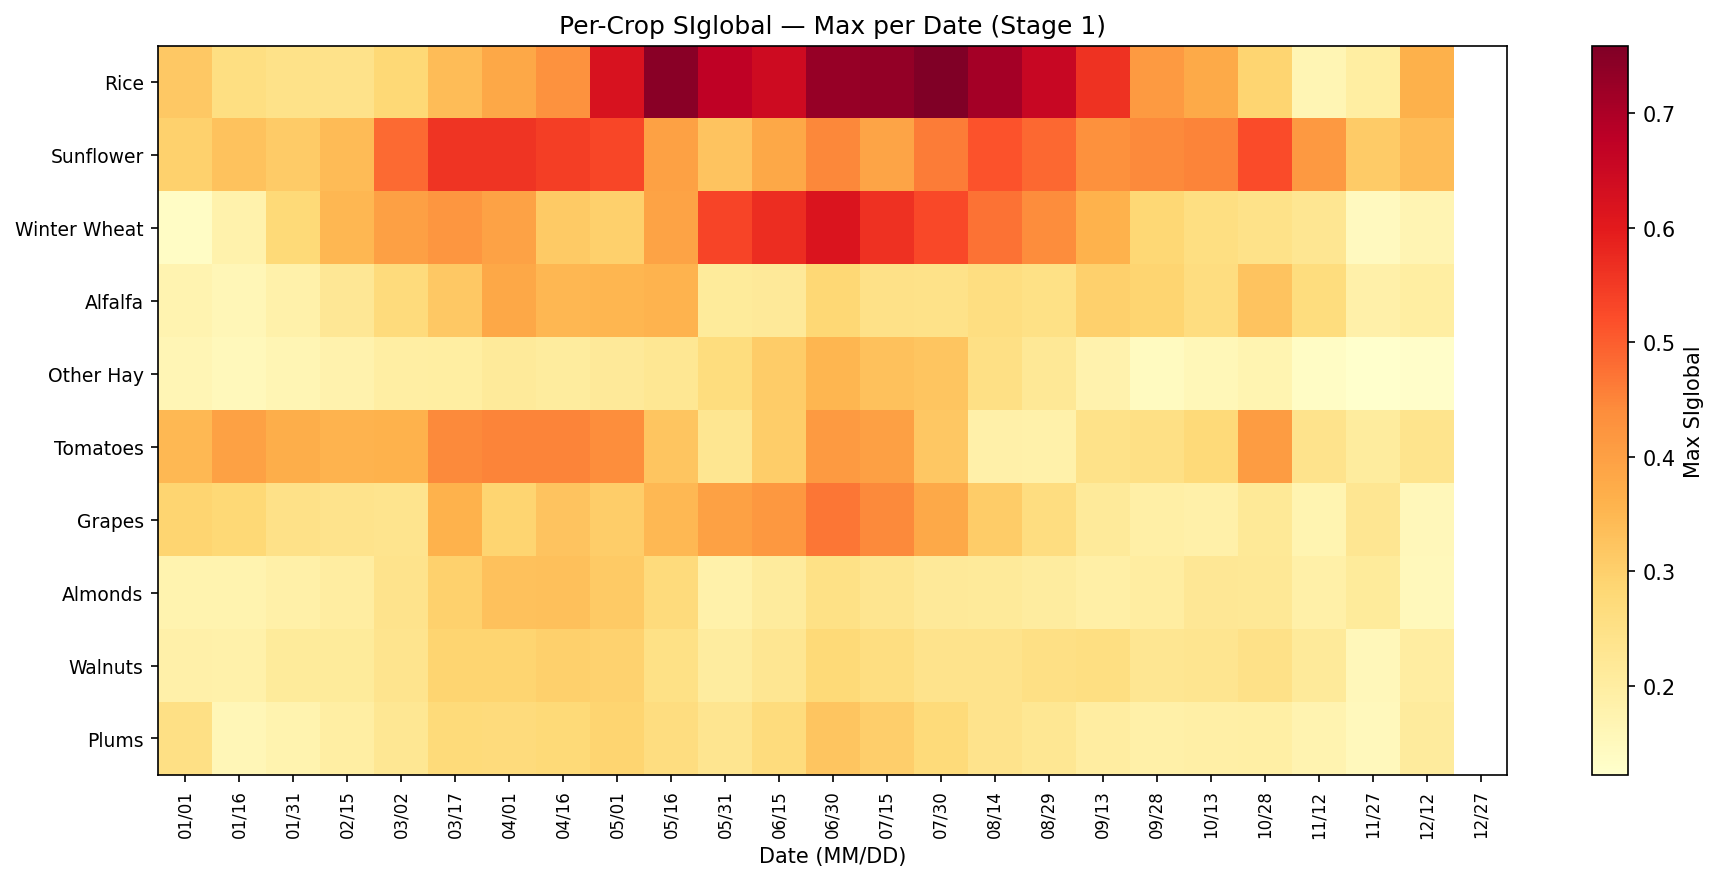
\includegraphics[width=0.95\textwidth]{figures/stage1v2_siglobal_heatmap.png}
    \caption{Tahap 1 --- Peta panas nilai GSI per \textit{band-date} per kelas tanaman.
             Band SWIR (B11, B12) dan \textit{Red Edge} (B5--B7) secara konsisten menunjukkan
             nilai tertinggi. Tanggal Oktober--Desember menonjol untuk tanaman pohon tahunan,
             sedangkan tanggal Juni--Juli dominan untuk tanaman semusim.}
    \label{fig:stage1v2_siglobal_heatmap}
\end{figure}

Berdasarkan peringkat GSI Tahap 1, tanggal terbaik per kelas tanaman (Phase A — \textit{band sweep})
adalah sebagai berikut:

\begin{table}[H]
    \centering
    \caption{Tanggal top-1 GSI dan band terbaik per kelas tanaman (Tahap 1, referensi 2022)}
    \label{tab:stage1_top_date}
    \begin{tabular}{|l|c|c|}
    \hline
    \textbf{Kelas Tanaman} & \textbf{Tanggal Top-1} & \textbf{Band Terbaik} \\
    \hline
    Rice          & 30 Juli 2022     & B12 \\
    Sunflower     & 28 Oktober 2022  & B8  \\
    Winter Wheat  & 27 Desember 2022 & B1  \\
    Alfalfa       & 1 April 2022     & B8A \\
    Other Hay     & 30 Juni 2022     & B11 \\
    Tomatoes      & 27 Desember 2022 & B1  \\
    Grapes        & 16 Mei 2022      & B11 \\
    Almonds       & 27 Desember 2022 & B1  \\
    Walnuts       & 28 Oktober 2022  & B6  \\
    Plums         & 30 Juni 2022     & B7  \\
    \hline
    \end{tabular}
\end{table}

Tabel~\ref{tab:stage1_top_date} menunjukkan bahwa tanaman pohon tahunan (\textit{Winter Wheat},
\textit{Almonds}, \textit{Tomatoes}) memiliki GSI tertinggi pada bulan Desember, bertepatan
dengan fase dorman musim dingin yang menciptakan kontras spektral tertinggi terhadap tanaman
lainnya yang masih aktif. \textit{Rice} memiliki puncak separabilitas pada Juli karena sinyal
unik dari fase penggenangan sawah, sedangkan \textit{Grapes} dan \textit{Alfalfa} mencapai
separabilitas tertinggi pada musim semi (April--Mei).

Jumlah channel setelah \textit{union} lintas semua kelas untuk masing-masing nilai $K$ disajikan
pada Tabel~\ref{tab:channel_counts}.

\begin{table}[H]
    \centering
    \caption{Jumlah channel setelah union lintas kelas untuk Phase A (band) dan Phase B (tanggal)}
    \label{tab:channel_counts}
    \begin{tabular}{|c|c|c|}
    \hline
    $K$ & \textbf{Phase A (ch)} & \textbf{Phase B (ch)} \\
    \hline
    1 & 8   & 59  \\
    2 & 17  & 107 \\
    3 & 25  & 147 \\
    4 & 33  & 189 \\
    5 & 39  & 212 \\
    \hline
    \end{tabular}
\end{table}

\subsection{Exp A\_v2 — Pengaruh Jendela Fenologi}

Eksperimen A\_v2 mengevaluasi dampak pemilihan jendela tanggal terhadap performa \textit{single-date}
dengan menggunakan tanggal akuisisi terdekat dari empat target fenologi: Januari (dorman),
Maret (musim semi), Juli (puncak musim panas), dan November (akhir musim).

\begin{table}[H]
    \centering
    \caption{Perbandingan performa Exp A\_v2 per jendela fenologi (9 channel, set uji 2024)}
    \label{tab:av2_results}
    \begin{tabular}{|l|l|c|c|c|}
    \hline
    \textbf{Jendela} & \textbf{Arsitektur} & \textbf{Val mIoU} & \textbf{Test mIoU} & \textbf{Test OA} \\
    \hline
    Januari  & SegFormer      & 0.3513 & 0.0215 & 0.0548 \\
    \hline
    Maret    & SegFormer      & 0.3128 & 0.1317 & 0.3800 \\
    Maret    & DeepLabV3+CBAM & 0.2990 & 0.0194 & 0.0612 \\
    \hline
    Juli     & SegFormer      & 0.4695 & 0.1816 & 0.4363 \\
    Juli     & DeepLabV3+CBAM & 0.4588 & 0.0421 & 0.2857 \\
    \hline
    November & SegFormer      & 0.3659 & 0.0775 & 0.1694 \\
    November & DeepLabV3+CBAM & 0.3531 & 0.0414 & 0.3113 \\
    \hline
    \end{tabular}
\end{table}

Tabel~\ref{tab:iou_av2_per_kelas} menampilkan IoU per kelas untuk SegFormer pada keempat jendela.

\begin{table}[H]
    \centering
    \caption{IoU per kelas Exp A\_v2 SegFormer per jendela fenologi (set uji 2024, \%)}
    \label{tab:iou_av2_per_kelas}
    \resizebox{\textwidth}{!}{%
    \begin{tabular}{|l|c|c|c|c|}
    \hline
    \textbf{Kelas} & \textbf{Januari} & \textbf{Maret} & \textbf{Juli} & \textbf{November} \\
    \hline
    Rice         & 2.56  & 35.16 & \textbf{38.54} & 23.23 \\
    Sunflower    & 0.08  & 4.38  & \textbf{18.34} & 1.41  \\
    Winter Wheat & 3.41  & \textbf{13.40} & 13.24 & 3.94  \\
    Alfalfa      & 2.06  & 11.47 & \textbf{18.18} & 9.09  \\
    Other Hay    & 1.19  & 1.22  & 0.88  & \textbf{1.01}  \\
    Tomatoes     & 3.56  & 7.84  & \textbf{20.82} & 9.00  \\
    Grapes       & 0.00  & 11.12 & \textbf{16.69} & 3.64  \\
    Almonds      & 4.60  & 29.91 & \textbf{32.21} & 10.42 \\
    Walnuts      & 2.91  & 16.77 & \textbf{21.52} & 14.95 \\
    Plums        & 1.13  & 0.38  & \textbf{1.17}  & 0.86  \\
    \hline
    \textbf{mIoU} & 2.15 & 13.17 & \textbf{18.16} & 7.75  \\
    \hline
    \end{tabular}%
    }
\end{table}

Dari Tabel~\ref{tab:av2_results} dan~\ref{tab:iou_av2_per_kelas}, diperoleh beberapa temuan penting:

\begin{enumerate}
    \item \textbf{Jendela Juli tetap dominan} dengan test mIoU terbaik (0.1816 untuk SegFormer),
    mengonfirmasi bahwa pemilihan tanggal 30 Juli pada Exp A awal didasarkan pada kualitas data
    yang juga bertepatan dengan puncak fenologi mayoritas tanaman target.

    \item \textbf{Jendela Maret menjadi runner-up} (SegFormer 0.1317), dan secara khusus
    mengungguli Juli untuk \textit{Winter Wheat} (13.40\% vs 13.24\%). Hal ini memvalidasi
    hipotesis fenologi: tanaman musim dingin yang sudah dipanen pada Juli lebih mudah dibedakan
    pada Maret ketika masih aktif tumbuh.

    \item \textbf{Jendela Januari bersifat destruktif} (0.0215) --- seluruh tanaman musim panas
    dalam kondisi dorman atau belum ditanam, sehingga sinyal spektral tidak membawa informasi
    diskriminatif yang cukup. Menggunakan Januari sebagai input tunggal secara signifikan
    menurunkan performa model.

    \item \textbf{SegFormer konsisten mengungguli DeepLabV3+CBAM} pada semua jendela untuk
    input \textit{single-date}, mengonfirmasi keunggulan \textit{self-attention} dalam
    menangkap konteks spasial dari input yang bersih dan tidak redundan.
\end{enumerate}

\subsection{Exp C\_v3 — Kurva K-Sweep}

\subsubsection{Phase A — Band Sweep}

Phase A mengevaluasi dampak menambah jumlah band ($K$) dari top-1 tanggal GSI per kelas tanaman.
Tabel~\ref{tab:cv3_band_results} merangkum hasil seluruh titik sweep.

\begin{table}[H]
    \centering
    \caption{Hasil Exp C\_v3 Phase A (\textit{band sweep}) pada set uji 2024}
    \label{tab:cv3_band_results}
    \begin{tabular}{|c|c|l|c|c|c|}
    \hline
    $K$ & \textbf{Ch.} & \textbf{Arsitektur} & \textbf{Val mIoU} & \textbf{Test mIoU} & \textbf{Test OA} \\
    \hline
    \multirow{2}{*}{1} & \multirow{2}{*}{8}  & SegFormer      & 0.4637 & 0.1122 & 0.3796 \\
                       &                     & DeepLabV3+CBAM & 0.4161 & 0.0777 & 0.1672 \\
    \hline
    \multirow{2}{*}{2} & \multirow{2}{*}{17} & SegFormer      & 0.4609 & 0.1199 & 0.3880 \\
                       &                     & DeepLabV3+CBAM & 0.4460 & 0.0942 & 0.3983 \\
    \hline
    \multirow{2}{*}{3} & \multirow{2}{*}{25} & SegFormer      & 0.4816 & 0.1155 & 0.3839 \\
                       &                     & DeepLabV3+CBAM & 0.4427 & 0.1126 & 0.3812 \\
    \hline
    \multirow{2}{*}{4} & \multirow{2}{*}{33} & SegFormer      & 0.4798 & 0.1205 & 0.3807 \\
                       &                     & DeepLabV3+CBAM & 0.4538 & 0.0981 & 0.3497 \\
    \hline
    \multirow{2}{*}{5} & \multirow{2}{*}{39} & \textbf{SegFormer}      & \textbf{0.4878} & \textbf{0.1305} & \textbf{0.3907} \\
                       &                     & DeepLabV3+CBAM & 0.4739 & 0.0902 & 0.2441 \\
    \hline
    \end{tabular}
\end{table}

\begin{table}[H]
    \centering
    \caption{IoU per kelas Phase A SegFormer (set uji 2024, \%)}
    \label{tab:cv3_band_per_kelas}
    \resizebox{\textwidth}{!}{%
    \begin{tabular}{|l|c|c|c|c|c|}
    \hline
    \textbf{Kelas} & $k$=1 (8ch) & $k$=2 (17ch) & $k$=3 (25ch) & $k$=4 (33ch) & $k$=5 (39ch) \\
    \hline
    Rice         & 34.70 & 34.76 & 34.72 & 34.95 & 34.92 \\
    Sunflower    & 6.29  & 8.38  & 8.07  & 8.44  & 10.72 \\
    Winter Wheat & 9.93  & 9.89  & 9.22  & 9.78  & 10.22 \\
    Alfalfa      & 6.35  & 8.04  & 7.56  & 10.77 & 11.46 \\
    Other Hay    & 1.09  & 1.02  & 0.97  & 0.94  & 1.36  \\
    Tomatoes     & 7.65  & 8.83  & 8.71  & 9.80  & 9.01  \\
    Grapes       & 9.97  & 10.07 & 8.73  & 6.17  & 9.15  \\
    Almonds      & 24.25 & 25.18 & 24.62 & 26.10 & 29.02 \\
    Walnuts      & 11.13 & 11.66 & 11.68 & 12.06 & 12.77 \\
    Plums        & 0.96  & 2.09  & 1.33  & 1.47  & 1.86  \\
    \hline
    \textbf{mIoU} & 11.22 & 11.99 & 11.55 & 12.05 & \textbf{13.05} \\
    \hline
    \end{tabular}%
    }
\end{table}

\subsubsection{Phase B — Date Sweep}

Phase B mengevaluasi dampak menambah jumlah tanggal ($K$) dengan seluruh 9 band.
Tabel~\ref{tab:cv3_date_results} merangkum hasil seluruh titik sweep.

\begin{table}[H]
    \centering
    \caption{Hasil Exp C\_v3 Phase B (\textit{date sweep}) pada set uji 2024}
    \label{tab:cv3_date_results}
    \begin{tabular}{|c|c|l|c|c|c|}
    \hline
    $K$ & \textbf{Ch.} & \textbf{Arsitektur} & \textbf{Val mIoU} & \textbf{Test mIoU} & \textbf{Test OA} \\
    \hline
    \multirow{2}{*}{1} & \multirow{2}{*}{59}  & SegFormer      & 0.4983 & 0.1250 & 0.3886 \\
                       &                      & DeepLabV3+CBAM & 0.5101 & 0.1027 & 0.1717 \\
    \hline
    \multirow{2}{*}{2} & \multirow{2}{*}{107} & SegFormer      & 0.4999 & 0.1317 & 0.3901 \\
                       &                      & DeepLabV3+CBAM & 0.5182 & 0.1284 & 0.3900 \\
    \hline
    \multirow{2}{*}{3} & \multirow{2}{*}{147} & SegFormer          & 0.5182 & 0.1333 & 0.3935 \\
                       &                      & \textbf{DeepLabV3+CBAM} & \textbf{0.5254} & \textbf{0.1353} & \textbf{0.3965} \\
    \hline
    \multirow{2}{*}{4} & \multirow{2}{*}{189} & SegFormer      & 0.5208 & 0.1326 & 0.3809 \\
                       &                      & DeepLabV3+CBAM & 0.5310 & 0.1136 & 0.4098 \\
    \hline
    \multirow{2}{*}{5} & \multirow{2}{*}{212} & SegFormer      & 0.5171 & 0.1355 & 0.3946 \\
                       &                      & DeepLabV3+CBAM & 0.5243 & 0.1339 & 0.4022 \\
    \hline
    \end{tabular}
\end{table}

\begin{table}[H]
    \centering
    \caption{IoU per kelas Phase B DeepLabV3+CBAM (set uji 2024, \%)}
    \label{tab:cv3_date_per_kelas}
    \resizebox{\textwidth}{!}{%
    \begin{tabular}{|l|c|c|c|c|c|}
    \hline
    \textbf{Kelas} & $k$=1 (59ch) & $k$=2 (107ch) & $k$=3 (147ch) & $k$=4 (189ch) & $k$=5 (212ch) \\
    \hline
    Rice         & 18.85 & 34.33 & \textbf{34.99} & 17.49 & 35.10 \\
    Sunflower    & 14.45 & 16.53 & \textbf{17.36} & 14.10 & 16.55 \\
    Winter Wheat & 9.59  & 9.87  & \textbf{11.38} & 10.72 & 10.61 \\
    Alfalfa      & 1.76  & 9.99  & \textbf{11.55} & 11.69 & 11.29 \\
    Other Hay    & 1.11  & 1.24  & 0.97  & 1.01  & 1.18  \\
    Tomatoes     & 9.75  & 9.23  & \textbf{9.46}  & 10.14 & 9.99  \\
    Grapes       & 9.83  & 10.03 & \textbf{9.85}  & 9.77  & 9.94  \\
    Almonds      & 24.96 & 23.81 & 24.18 & 24.59 & \textbf{25.05} \\
    Walnuts      & 11.12 & 11.93 & \textbf{13.67} & 12.85 & 13.21 \\
    Plums        & 1.28  & 1.44  & \textbf{1.94}  & 1.19  & 0.98  \\
    \hline
    \textbf{mIoU} & 10.27 & 12.84 & \textbf{13.53} & 11.36 & 13.39 \\
    \hline
    \end{tabular}%
    }
\end{table}

\section{Analisis Hasil}

\subsection{Perbandingan Antar Konfigurasi Input}

Berdasarkan seluruh hasil eksperimen, diperoleh tiga temuan utama yang menjawab
pertanyaan penelitian secara bertahap:

\begin{enumerate}
    \item \textbf{Pengaruh jendela fenologi terhadap \textit{single-date}} (A vs.\ A\_v2):
    Jendela Juli terbukti optimal (SegFormer 0.1816 vs.\ Maret 0.1317 vs.\ November 0.0775 vs.\ Januari 0.0215).
    Pemilihan 30 Juli pada Exp A awal divalidasi sebagai pilihan yang tepat --- bukan hanya
    karena kualitas data (99,6\% valid pixels) tetapi juga karena bertepatan dengan puncak
    vegetasi mayoritas tanaman target.
    Satu-satunya pengecualian adalah \textit{Winter Wheat}: jendela Maret (13,40\%) sedikit
    mengungguli Juli (13,24\%), sesuai dengan siklus tanamnya yang aktif pada musim semi dan
    sudah dipanen pada bulan Juli.

    \item \textbf{Pengaruh multi-temporal} (A vs.\ B vs.\ C\_v3):
    Exp B naif (36 ch, SF 0.1017) tidak mampu melampaui Exp A (9 ch, SF 0.1937), mengindikasikan
    bahwa penambahan informasi temporal tanpa seleksi memperkenalkan \textit{noise} yang merugikan
    SegFormer. Namun, C\_v3 Phase B dengan $k$=3 (147 ch) mencapai test mIoU 0.1353 pada
    DeepLabV3+CBAM --- mendekati performa terbaik SegFormer pada Exp A.

    \item \textbf{Elbow kurva K-sweep} (C\_v3):
    Phase B (date sweep) mencapai titik \textit{elbow} pada $k$=3 (147 channel), di mana
    penambahan tanggal lebih lanjut tidak lagi meningkatkan test mIoU secara konsisten.
    Phase A (band sweep) terus meningkat hingga $k$=5 (39 channel) namun tetap di bawah
    performa Phase B --- mengindikasikan bahwa diversitas temporal lebih informatif daripada
    diversitas band pada tanggal terbaik saja.
\end{enumerate}

\subsection{Perbandingan Performa Arsitektur}

Dua pola arsitektur yang berbeda teridentifikasi dari eksperimen ini:

\begin{enumerate}
    \item \textbf{SegFormer unggul pada input \textit{single-date}}:
    Mekanisme \textit{self-attention} pada SegFormer mampu menangkap hubungan spasial jarak
    jauh secara efektif ketika input bersih (9 channel). Penambahan channel (Exp B, C\_v3 Phase A)
    tidak memberikan keunggulan bagi SegFormer, bahkan cenderung stagnan, karena
    \textit{self-attention} tidak memiliki mekanisme seleksi channel bawaan yang sesuai.

    \item \textbf{DeepLabV3+CBAM unggul pada input multi-temporal}:
    Modul CBAM (\textit{Channel Attention}) secara eksplisit memberikan bobot per channel,
    memungkinkan model untuk secara selektif mengabaikan channel yang tidak informatif.
    Hal ini menjelaskan mengapa DeepLabV3+CBAM menjadi kompetitif pada Phase B $k$=3
    (0.1353) --- setara dengan SegFormer terbaik (0.1355) meskipun menggunakan arsitektur
    berbasis CNN.
    Sebaliknya, DeepLabV3+CBAM sangat terbatas pada input \textit{single-date} (0.0511),
    karena CBAM dirancang untuk mengeksploitasi variasi antar channel.
\end{enumerate}

\subsection{Diskusi: Hipotesis Kombinasi Band dan Domain Shift}

Hasil pengujian menunjukkan bahwa performa terbaik secara keseluruhan diraih oleh
Exp A SegFormer (mIoU = 0.1937) menggunakan input \textit{single-date} yang tidak melibatkan
seleksi band multi-temporal.
Hal ini secara superfisial tampak bertentangan dengan hipotesis penelitian bahwa kombinasi
band multi-temporal akan meningkatkan akurasi.

Namun, terdapat dua faktor yang perlu dipertimbangkan dalam menginterpretasikan hasil ini:

\textbf{Pertama, \textit{temporal domain shift}.}
Evaluasi dilakukan pada tahun 2024 (independen), sedangkan model dilatih pada 2022--2023.
Gap yang besar antara val mIoU ($\approx$0.51--0.53 untuk C\_v3 Phase B) dan test mIoU
($\approx$0.13--0.14) mengindikasikan bahwa pergeseran fenologi antar tahun merupakan
tantangan utama, bukan kualitas metode seleksi band.
Model dengan input \textit{single-date} (Exp A) lebih tahan terhadap domain shift karena
hanya bergantung pada satu jendela waktu yang relatif stabil antar tahun (puncak vegetasi Juli),
sedangkan model multi-temporal bergantung pada profil temporal lengkap yang lebih rentan
terhadap pergeseran kalender tanam.

\textbf{Kedua, efek arsitektur.}
Hipotesis terbukti secara parsial bergantung pada arsitektur:
untuk DeepLabV3+CBAM, C\_v3 Phase B $k$=3 (0.1353) meningkat sebesar 165\% dibandingkan
Exp A (0.0511), memvalidasi bahwa seleksi band multi-temporal secara signifikan membantu
model berbasis CNN dengan mekanisme \textit{channel attention}.
SegFormer tidak mendapat manfaat yang sama karena arsitekturnya lebih optimal untuk input
berdimensi rendah yang bersih.

Temuan ini menghasilkan kesimpulan yang lebih bernuansa: \textit{efektivitas kombinasi band
multi-temporal bergantung pada arsitektur model dan stabilitas fenologi lintas tahun}.
Pada kondisi evaluasi lintas tahun (2022--2023 $\to$ 2024), kelebihan metode seleksi band
lebih terlihat pada model CNN dibandingkan Transformer.

\subsection{Proyeksi Band Antar-Tahun}

Band-band terpilih yang disimpan dalam format \texttt{BAND\_YYYYMMDD} diproyeksikan ke
tanggal akuisisi terdekat pada tahun 2023 (pelatihan) dan 2024 (pengujian) berdasarkan
\textit{Day-of-Year} (DOY):

\begin{equation}
    d^*(b, y) = \underset{d \in D_y}{\arg\min}\; \left| \text{DOY}(d) - \text{DOY}(\text{ref}_b) \right|
\end{equation}

Pergeseran tanggal hasil proyeksi umumnya hanya satu hari (akibat tahun kabisat atau
variasi jadwal akuisisi Sentinel-2), menjamin konsistensi informasi fenologi antar tahun.

\subsection{Analisis Kesalahan dan Keterbatasan}

Rendahnya nilai mIoU pada set uji 2024 dapat dijelaskan melalui tiga faktor utama:

\begin{enumerate}
    \item \textbf{\textit{Static Label vs.\ Dynamic Reality}}:
    Label CDL bersifat tahunan --- satu piksel diberi label tetap (misalnya ``\textit{Rice}'')
    untuk seluruh tahun, meskipun secara biofisik piksel tersebut hanya tampak sebagai padi
    selama fase vegetatif (Mei--September). Model yang dilatih pada fitur multi-temporal
    akan dipenalti oleh metrik IoU saat memprediksi \textit{background} pada tanggal di
    mana tanaman belum tumbuh atau sudah dipanen, meskipun prediksi tersebut secara
    biofisik benar.

    \item \textbf{\textit{Phenological Shift}}:
    Variasi cuaca antar tahun dapat menyebabkan pergeseran jadwal tanam atau panen.
    Pergeseran dua minggu antara tahun 2022 dan 2024 sudah cukup untuk mengubah
    fase pertumbuhan pada tanggal proyeksi yang sama, menyebabkan misklasifikasi
    pada model yang bergantung pada urutan temporal yang kaku.

    \item \textbf{Sensitivitas Kelas Minoritas}:
    Kelas dengan cakupan kecil seperti \textit{Other Hay} (1,4\%) dan \textit{Plums} (2,1\%)
    secara konsisten menunjukkan IoU mendekati nol di semua konfigurasi, mengindikasikan
    bahwa ketidakseimbangan kelas yang ekstrem tidak sepenuhnya teratasi oleh
    \textit{weighted loss} saja.
\end{enumerate}

\subsection{Waktu Pelatihan}

Tabel~\ref{tab:waktu_pelatihan} merangkum jumlah epoch yang diselesaikan untuk setiap
eksperimen berdasarkan log MLflow.

\begin{table}[H]
    \centering
    \caption{Epoch total per eksperimen (berdasarkan early stopping, max 100 epoch)}
    \label{tab:waktu_pelatihan}
    \begin{tabular}{|l|l|c|c|}
    \hline
    \textbf{Eksperimen} & \textbf{Arsitektur} & \textbf{Ch.} & \textbf{Epoch Total} \\
    \hline
    Exp A\_v2\_Jan  & SegFormer      & 9   & $\approx$100 \\
    Exp A\_v2\_Mar  & SegFormer      & 9   & $\approx$100 \\
    Exp A\_v2\_Jul  & SegFormer      & 9   & $\approx$100 \\
    Exp A\_v2\_Nov  & SegFormer      & 9   & $\approx$100 \\
    C\_v3 Band $k$=1 & SegFormer     & 8   & $\approx$100 \\
    C\_v3 Band $k$=5 & SegFormer     & 39  & $\approx$100 \\
    C\_v3 Date $k$=1 & DeepLabV3+    & 59  & $\approx$100 \\
    C\_v3 Date $k$=3 & DeepLabV3+    & 147 & 81 \\
    C\_v3 Date $k$=5 & SegFormer     & 212 & 81 \\
    \hline
    \end{tabular}
\end{table}

Semua eksperimen dihentikan melalui mekanisme \textit{early stopping} saat mIoU validasi
tidak meningkat lebih dari $\delta = 0.001$ dalam 20 epoch berturut-turut,
atau setelah mencapai batas maksimum 100 epoch.

\subsection{Visualisasi Kurva Pelatihan}

Gambar~\ref{fig:training_curves_dlv3} dan Gambar~\ref{fig:training_curves_sf}
menampilkan kurva \textit{loss} dan mIoU validasi selama pelatihan untuk
arsitektur DeepLabV3+CBAM dan SegFormer pada konfigurasi representatif.

\begin{figure}[H]
    \centering
    \begin{subfigure}{0.85\textwidth}
        \centering
        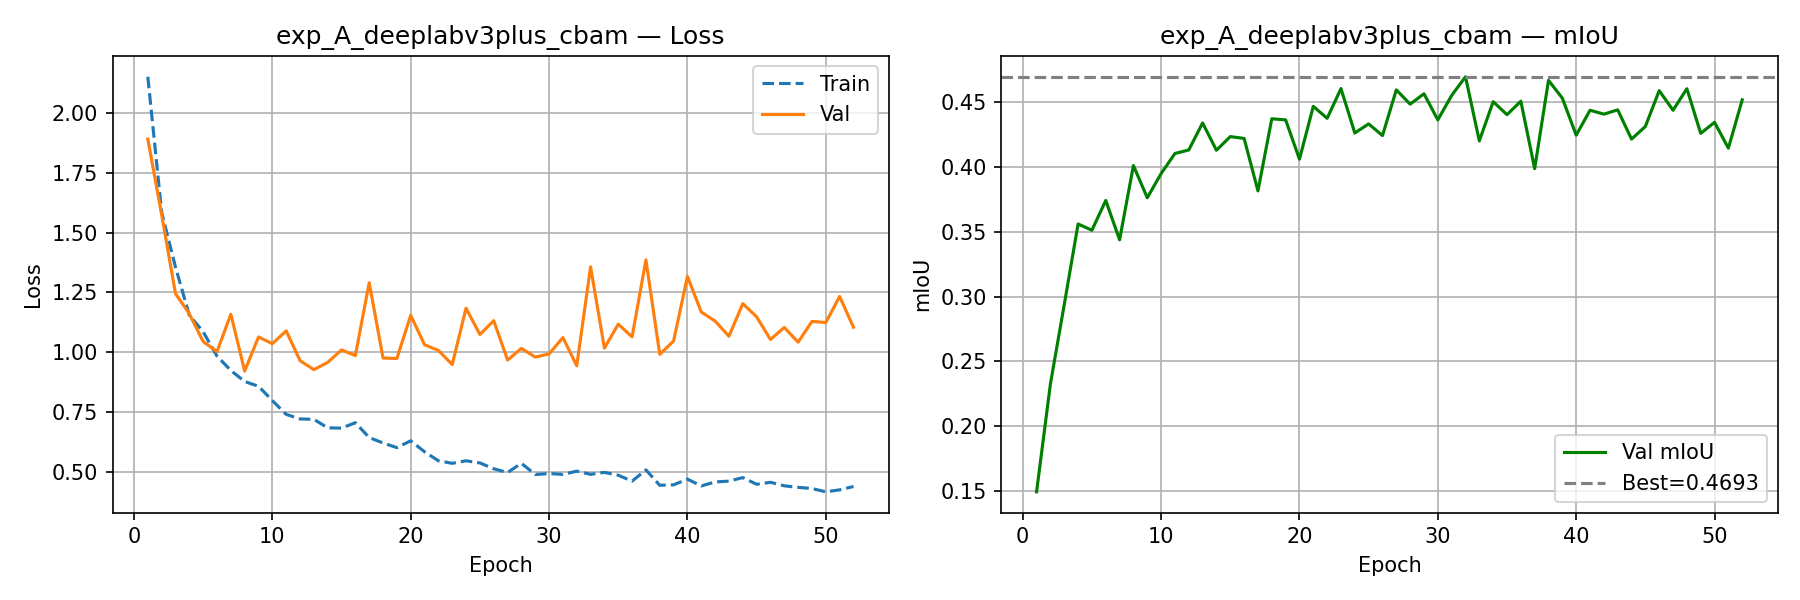
\includegraphics[width=\textwidth]{figures/dlv3_expa_curve.png}
        \caption{Exp A --- \textit{Single-Date} (9 ch)}
    \end{subfigure}
    \vspace{1em}
    \begin{subfigure}{0.85\textwidth}
        \centering
        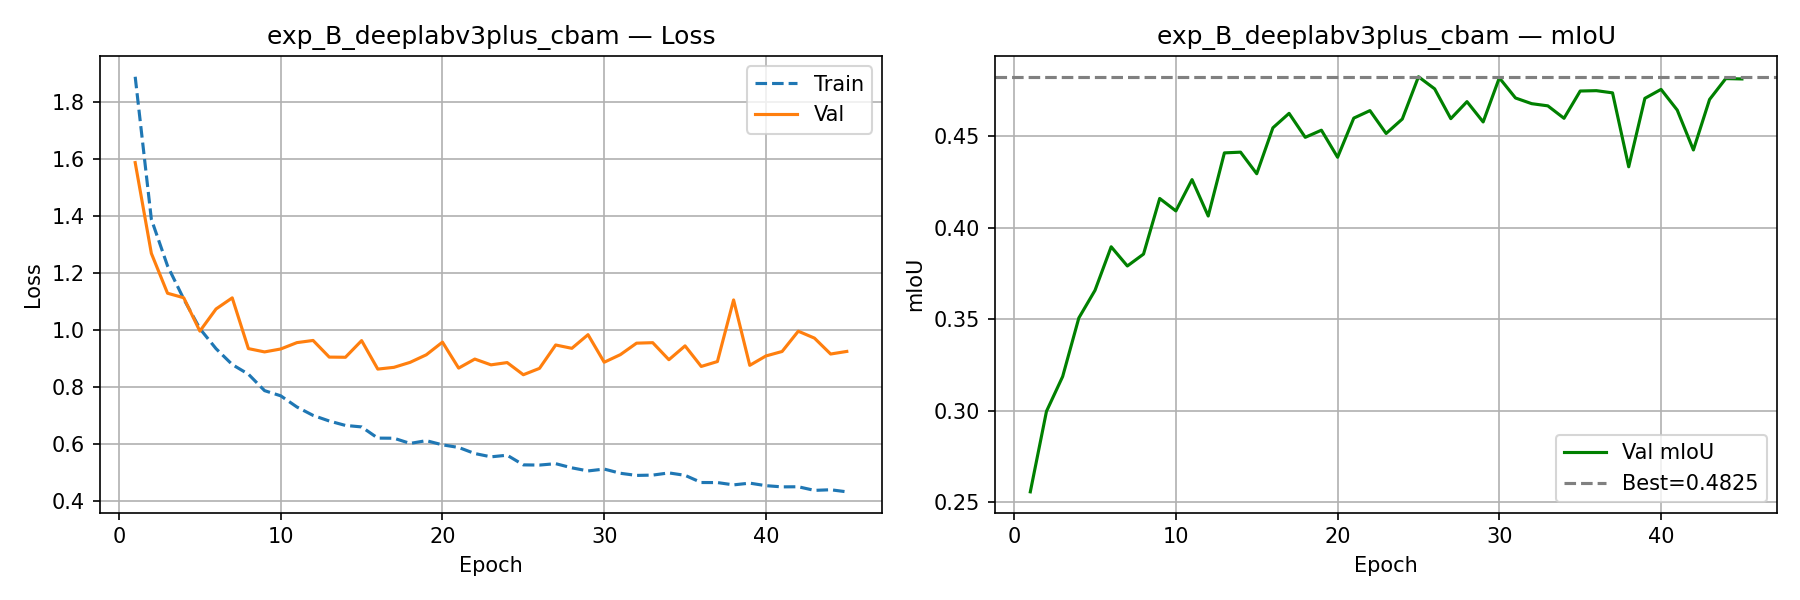
\includegraphics[width=\textwidth]{figures/dlv3_expb_curve.png}
        \caption{Exp B --- \textit{Multi-Temporal} Naif (36 ch)}
    \end{subfigure}
    \vspace{1em}
    \begin{subfigure}{0.85\textwidth}
        \centering
        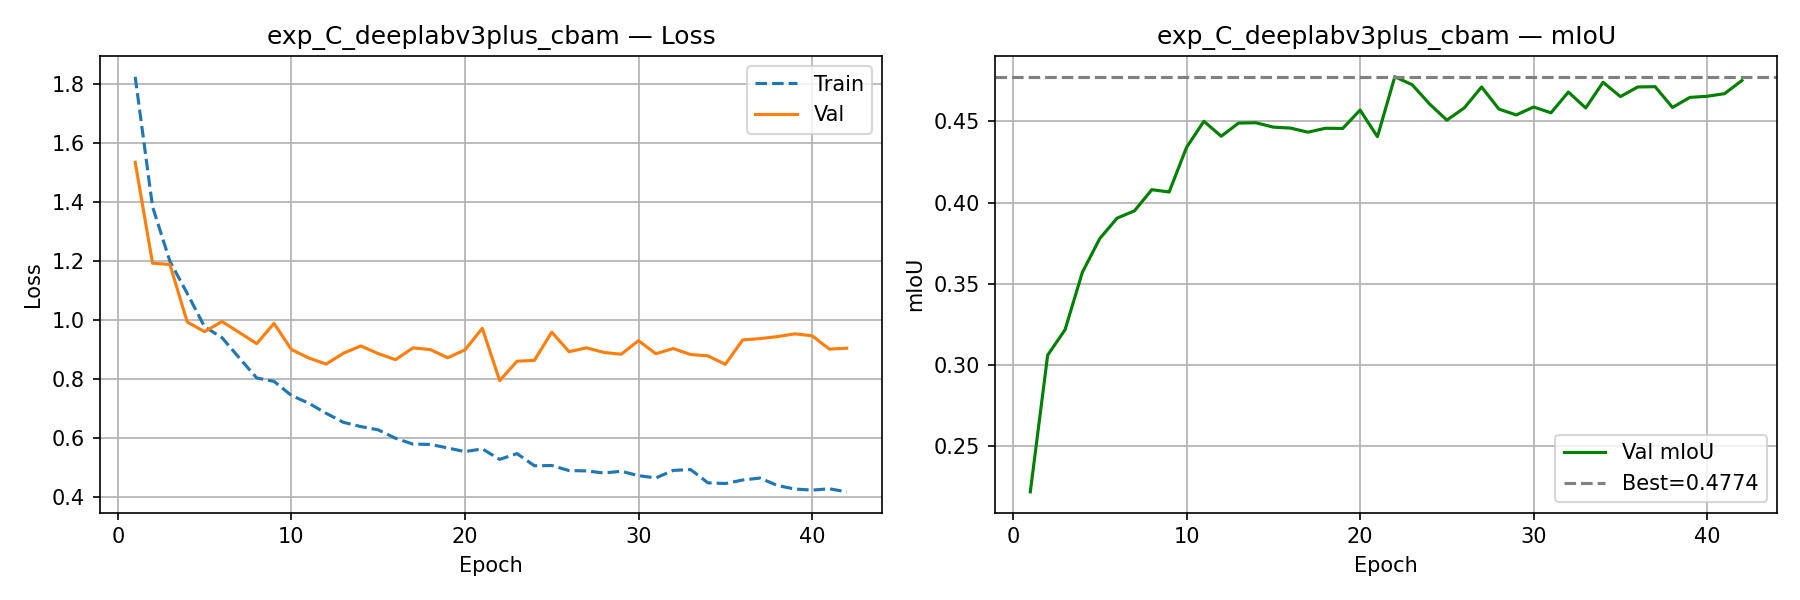
\includegraphics[width=\textwidth]{figures/dlv3_expc_curve.png}
        \caption{Exp C\_v3 --- Date $k$=3 (147 ch, \textit{best C\_v3})}
    \end{subfigure}
    \caption{Kurva pelatihan DeepLabV3+CBAM untuk konfigurasi representatif.}
    \label{fig:training_curves_dlv3}
\end{figure}

\begin{figure}[H]
    \centering
    \begin{subfigure}{0.85\textwidth}
        \centering
        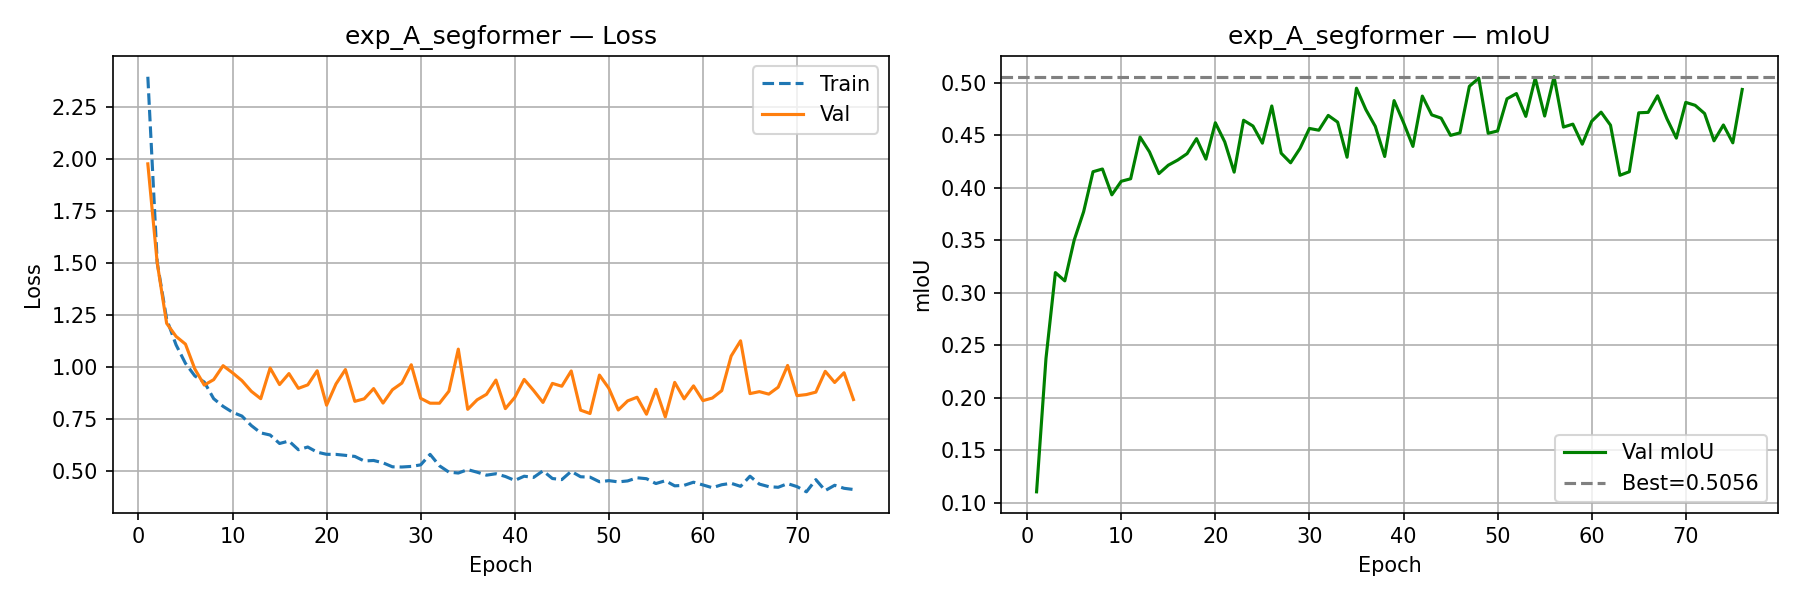
\includegraphics[width=\textwidth]{figures/sf_expa_curve.png}
        \caption{Exp A --- \textit{Single-Date} (9 ch)}
    \end{subfigure}
    \vspace{1em}
    \begin{subfigure}{0.85\textwidth}
        \centering
        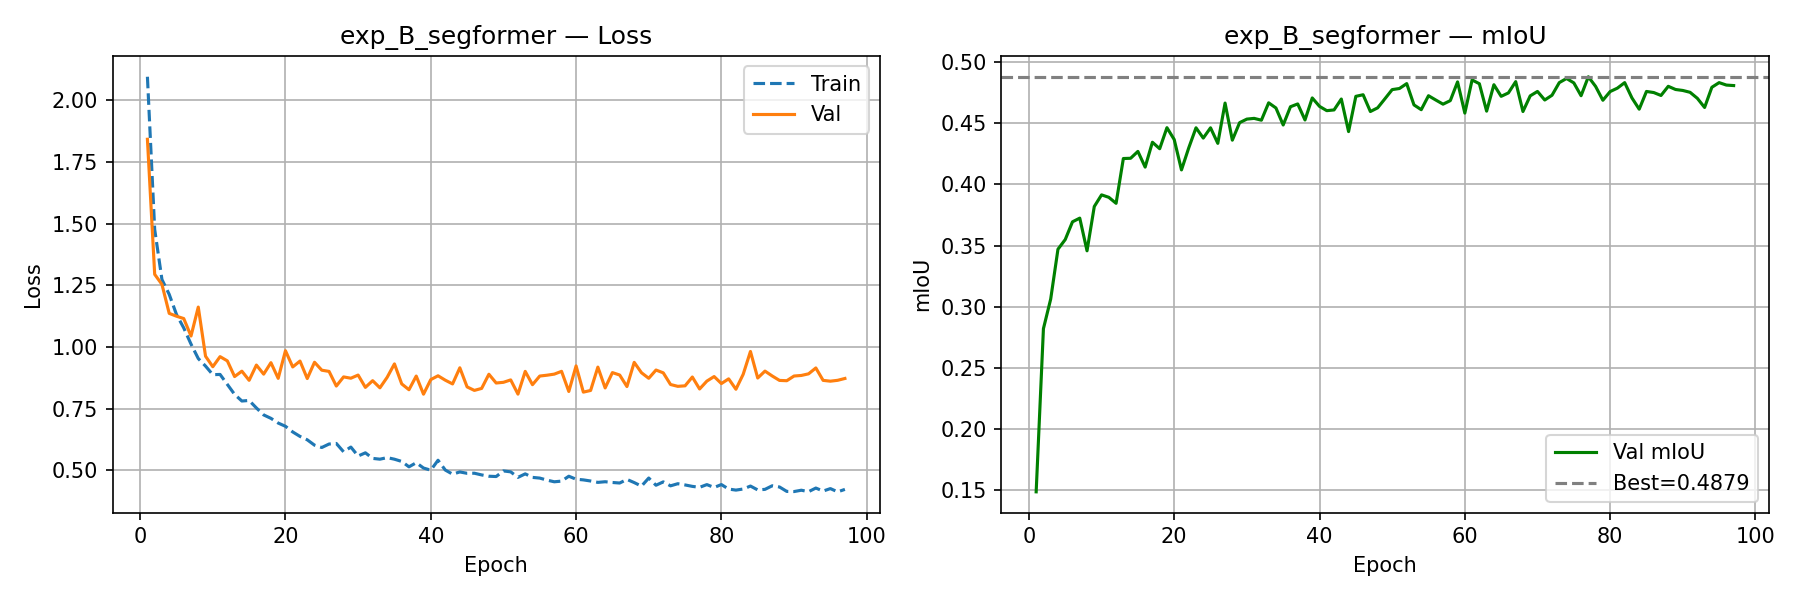
\includegraphics[width=\textwidth]{figures/sf_expb_curve.png}
        \caption{Exp B --- \textit{Multi-Temporal} Naif (36 ch)}
    \end{subfigure}
    \vspace{1em}
    \begin{subfigure}{0.85\textwidth}
        \centering
        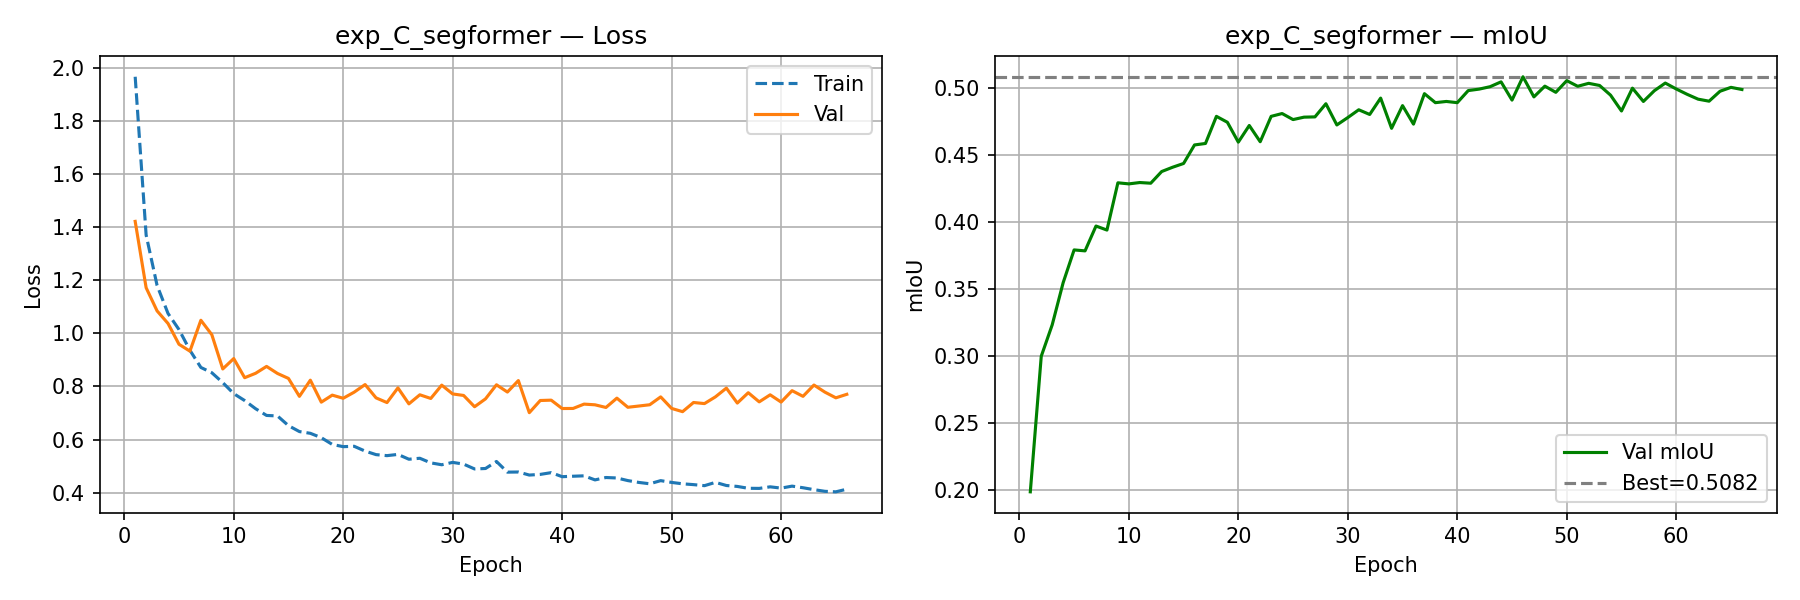
\includegraphics[width=\textwidth]{figures/sf_expc_curve.png}
        \caption{Exp C\_v3 --- Band $k$=5 (39 ch, \textit{best Phase A})}
    \end{subfigure}
    \caption{Kurva pelatihan SegFormer untuk konfigurasi representatif.}
    \label{fig:training_curves_sf}
\end{figure}

\subsection{Visualisasi Hasil Segmentasi}

Gambar~\ref{fig:seg_results_dlv3} dan Gambar~\ref{fig:seg_results_sf} menampilkan
peta segmentasi hasil inferensi penuh pada area studi Sacramento Valley menggunakan
data set uji tahun 2024.

\begin{figure}[H]
    \centering
    \begin{subfigure}{0.85\textwidth}
        \centering
        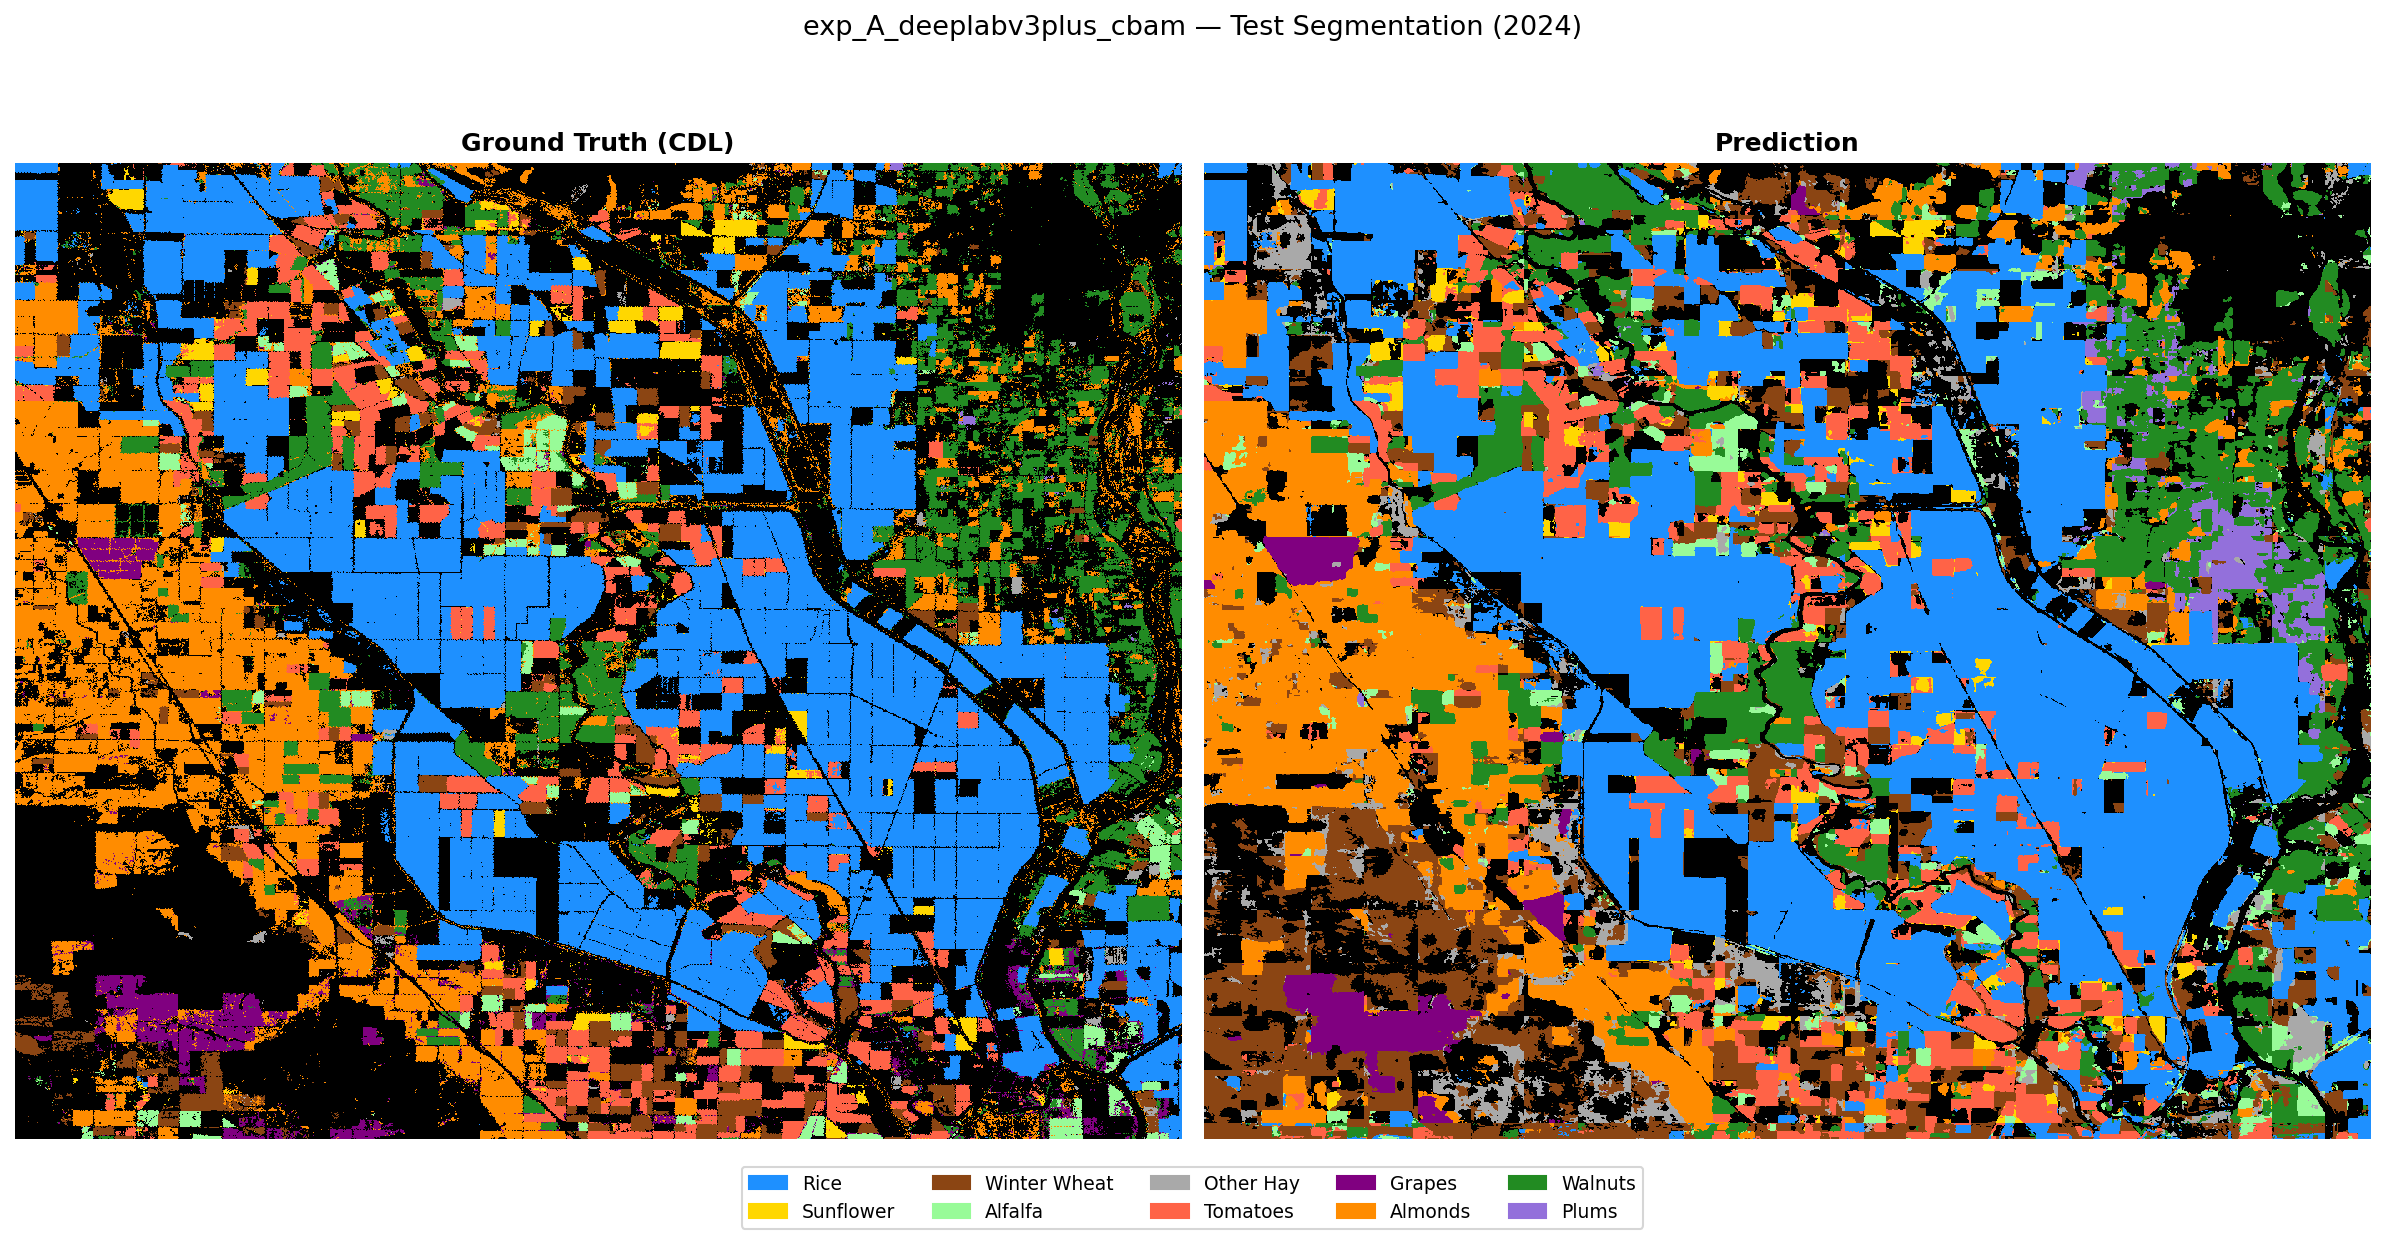
\includegraphics[width=\textwidth]{figures/dlv3_expa_map.png}
        \caption{Exp A --- \textit{Single-Date} (9 ch)}
    \end{subfigure}
    \vspace{1em}
    \begin{subfigure}{0.85\textwidth}
        \centering
        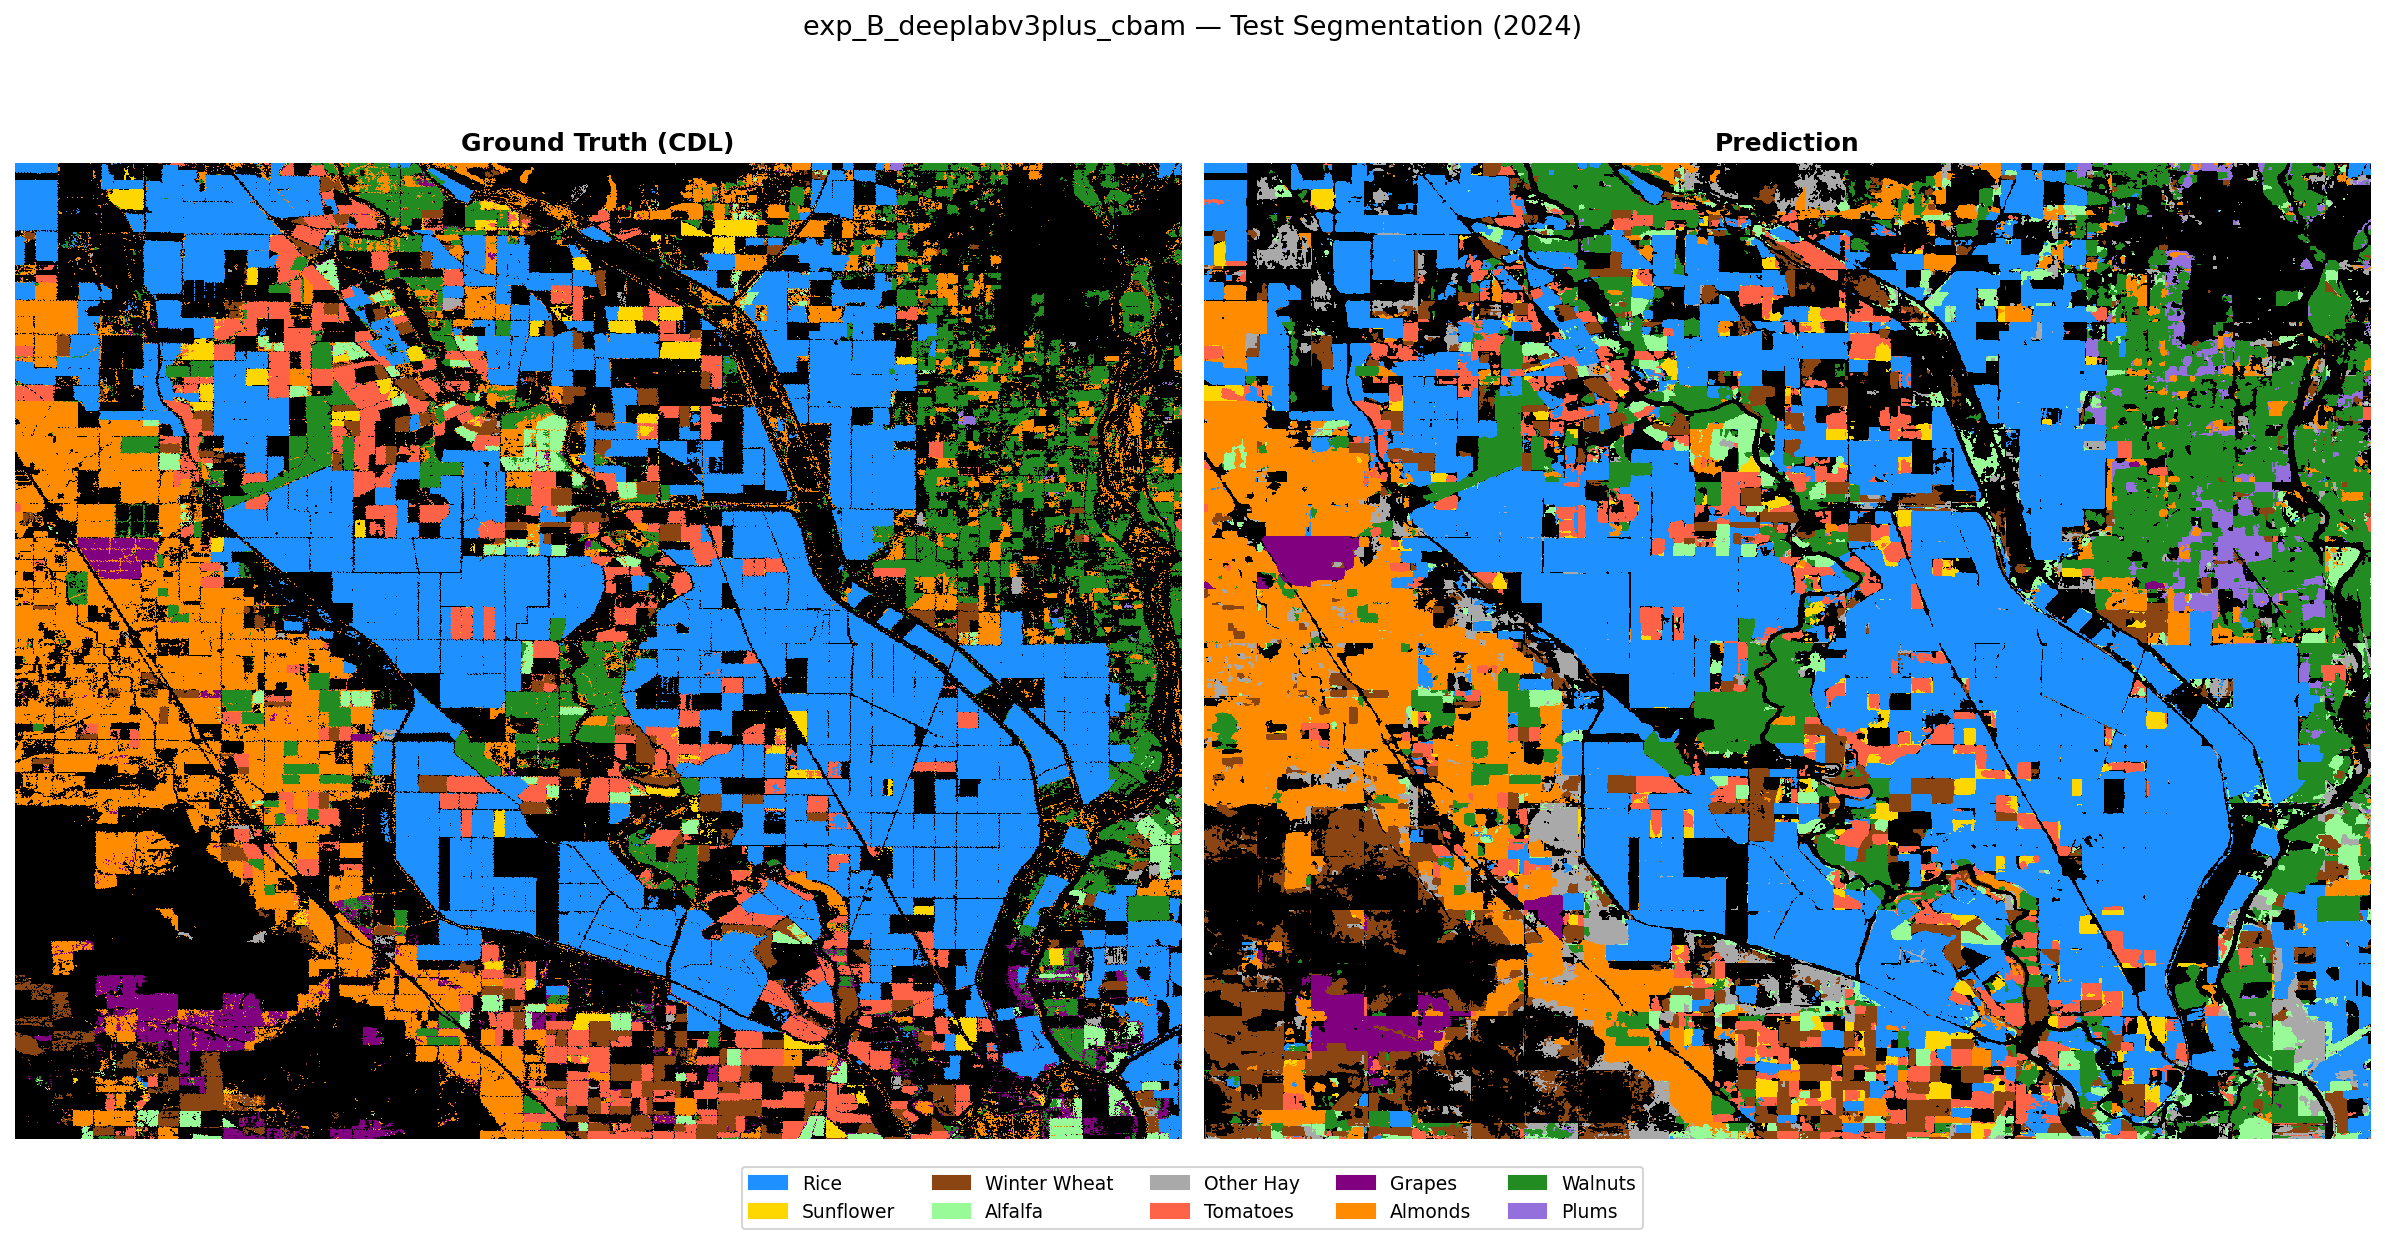
\includegraphics[width=\textwidth]{figures/dlv3_expb_map.png}
        \caption{Exp B --- \textit{Multi-Temporal} Naif (36 ch)}
    \end{subfigure}
    \vspace{1em}
    \begin{subfigure}{0.85\textwidth}
        \centering
        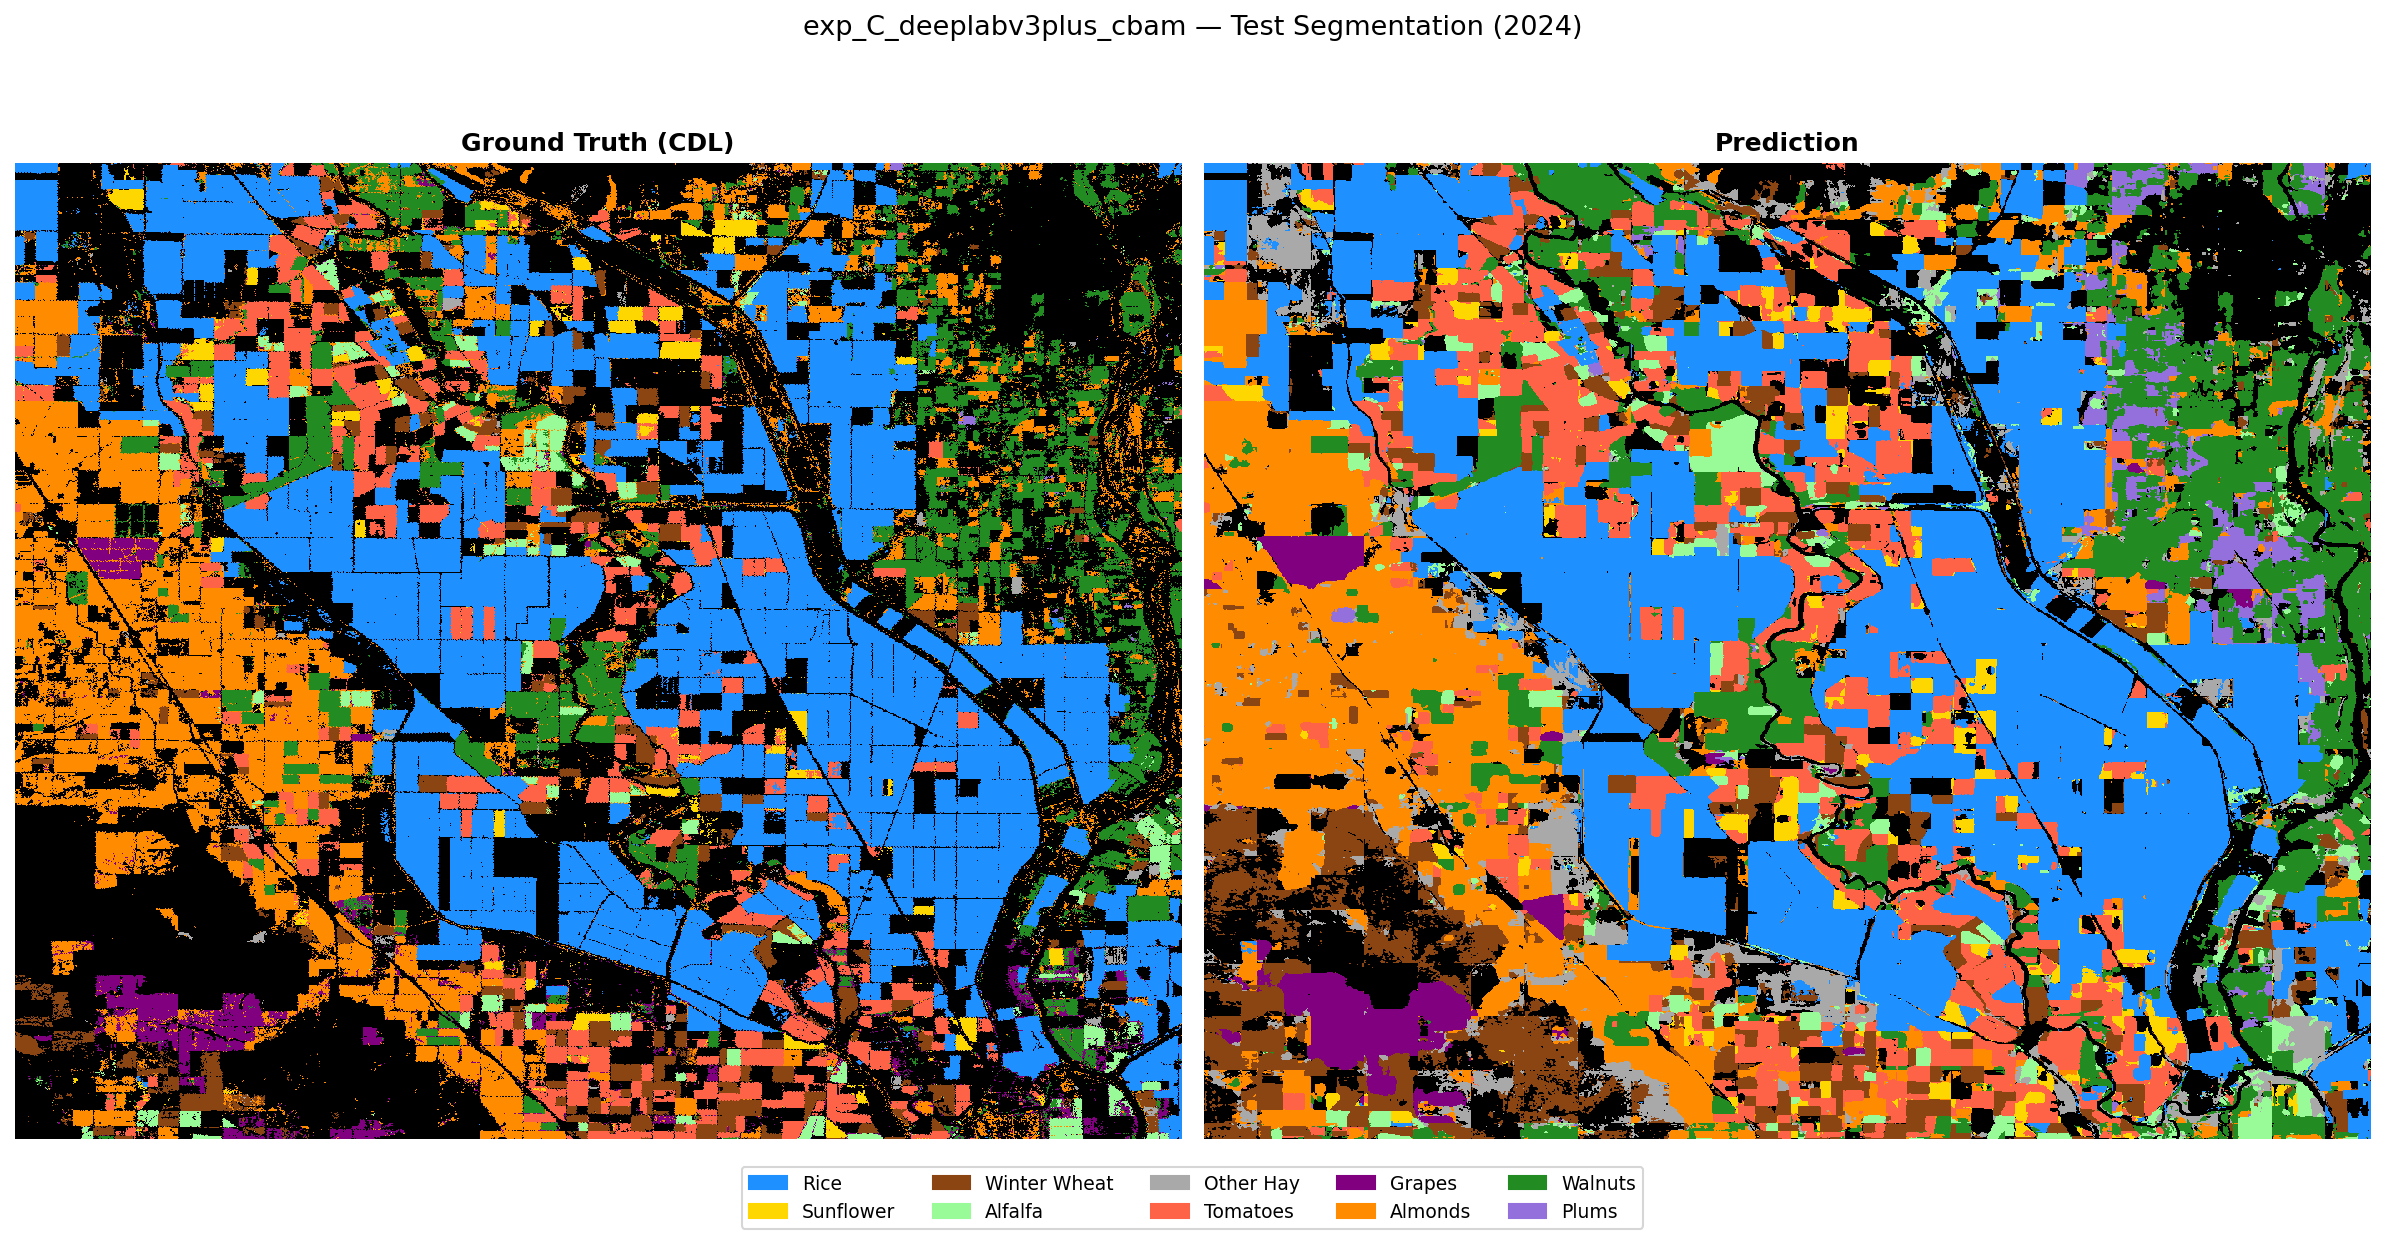
\includegraphics[width=\textwidth]{figures/dlv3_expc_map.png}
        \caption{Exp C\_v3 --- Date $k$=3 (147 ch, DeepLabV3+CBAM terbaik)}
    \end{subfigure}
    \caption{Peta segmentasi penuh set uji 2024 menggunakan DeepLabV3+CBAM.}
    \label{fig:seg_results_dlv3}
\end{figure}

\begin{figure}[H]
    \centering
    \begin{subfigure}{0.85\textwidth}
        \centering
        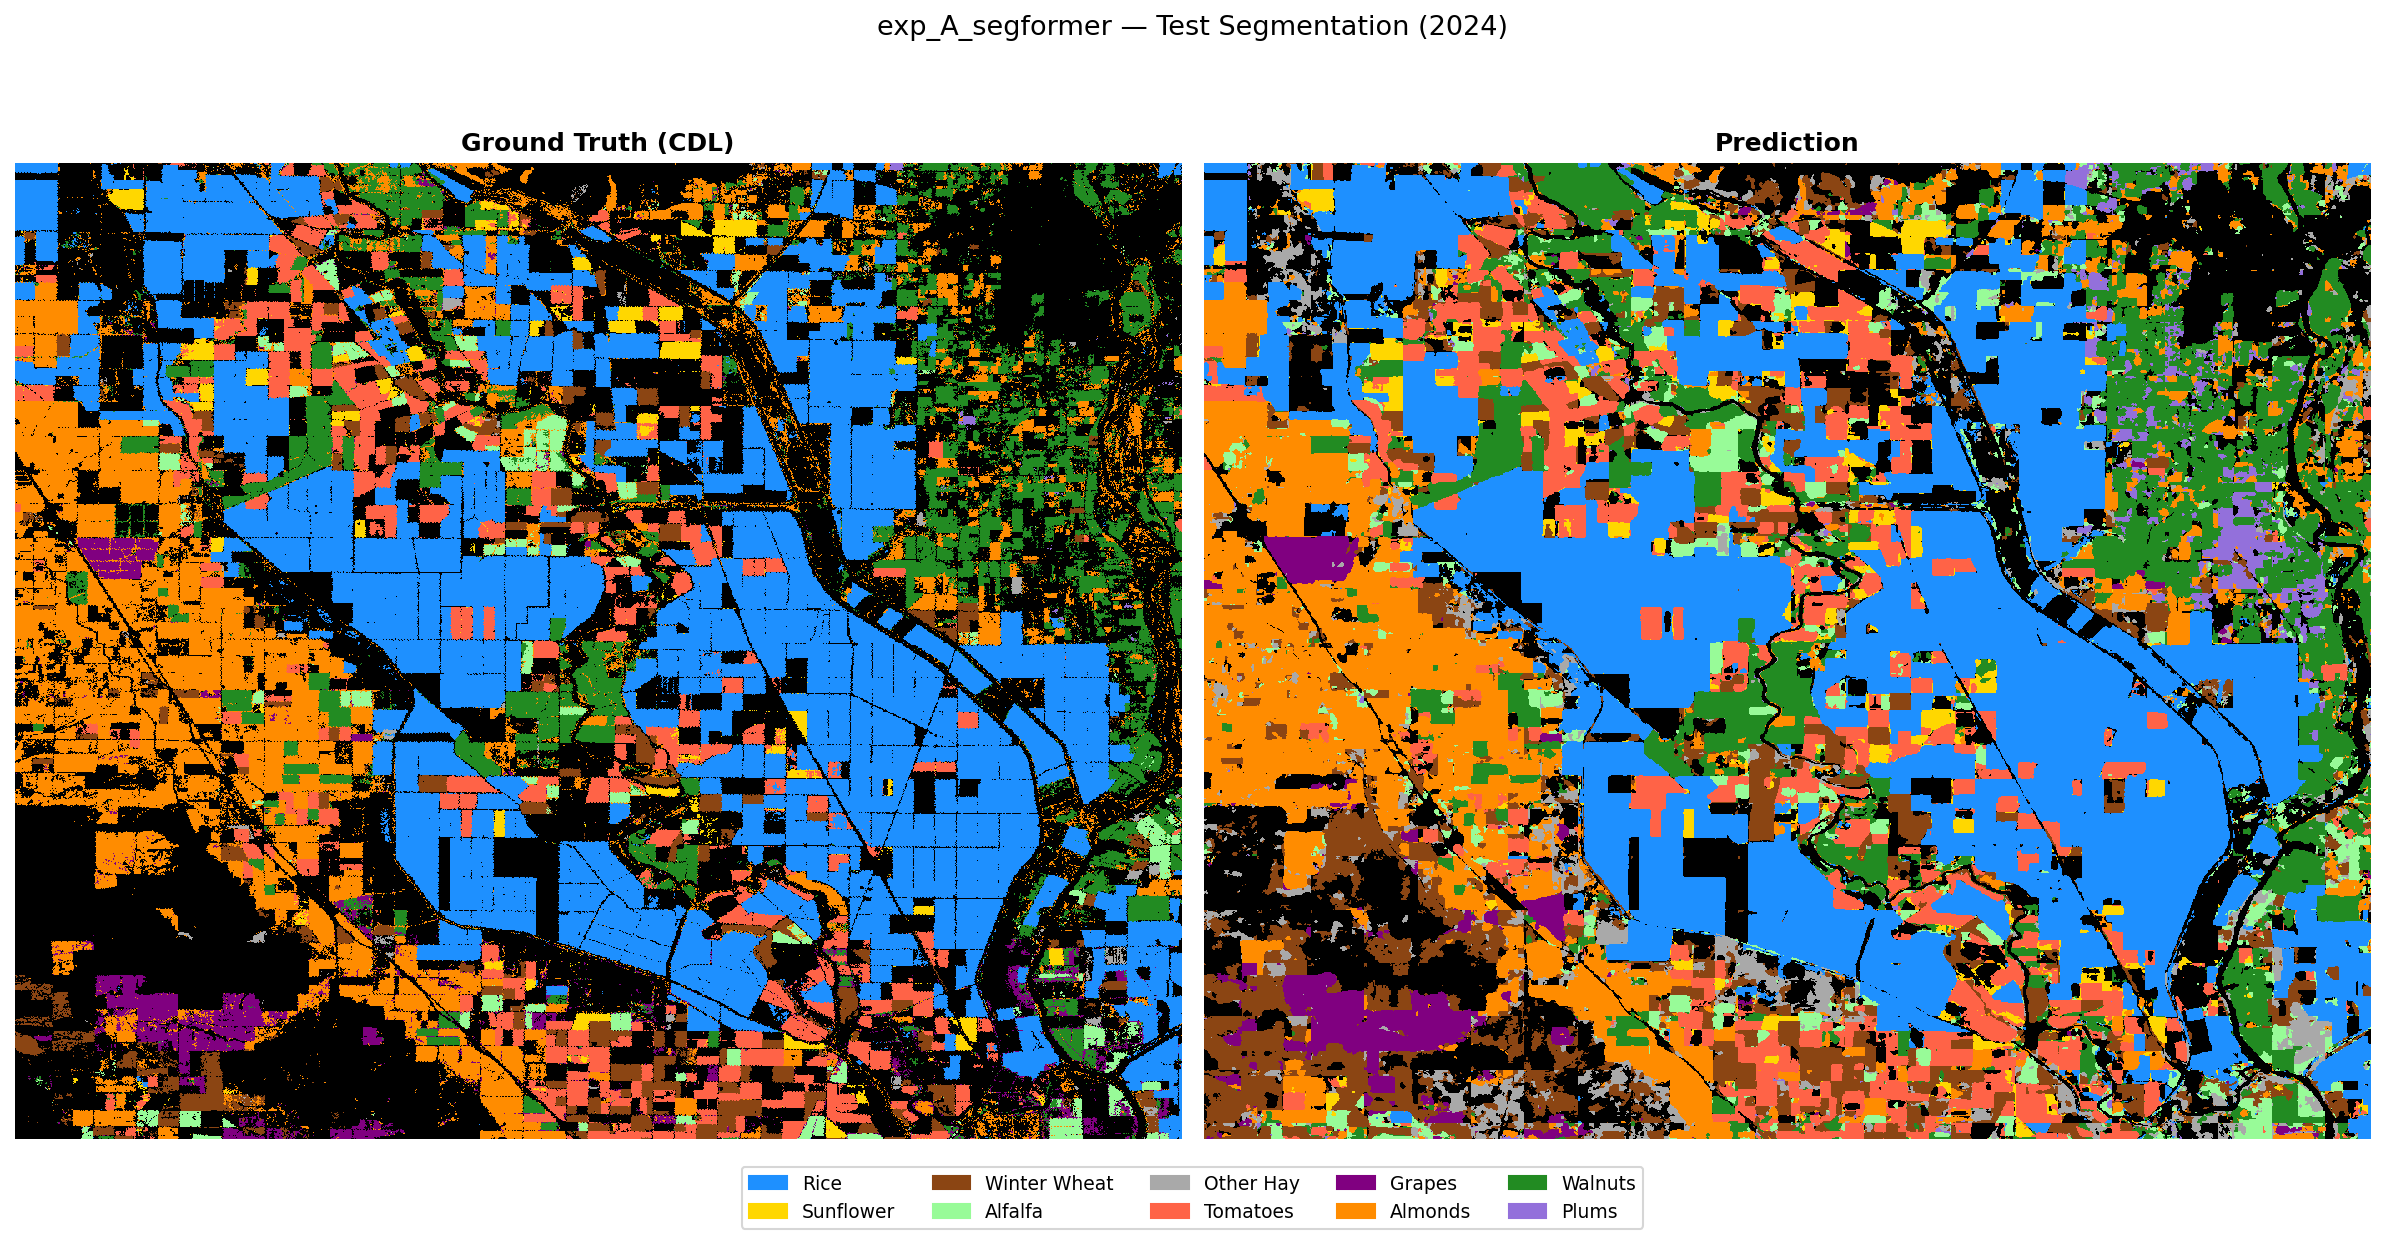
\includegraphics[width=\textwidth]{figures/sf_expa_map.png}
        \caption{Exp A --- \textit{Single-Date} (9 ch)}
    \end{subfigure}
    \vspace{1em}
    \begin{subfigure}{0.85\textwidth}
        \centering
        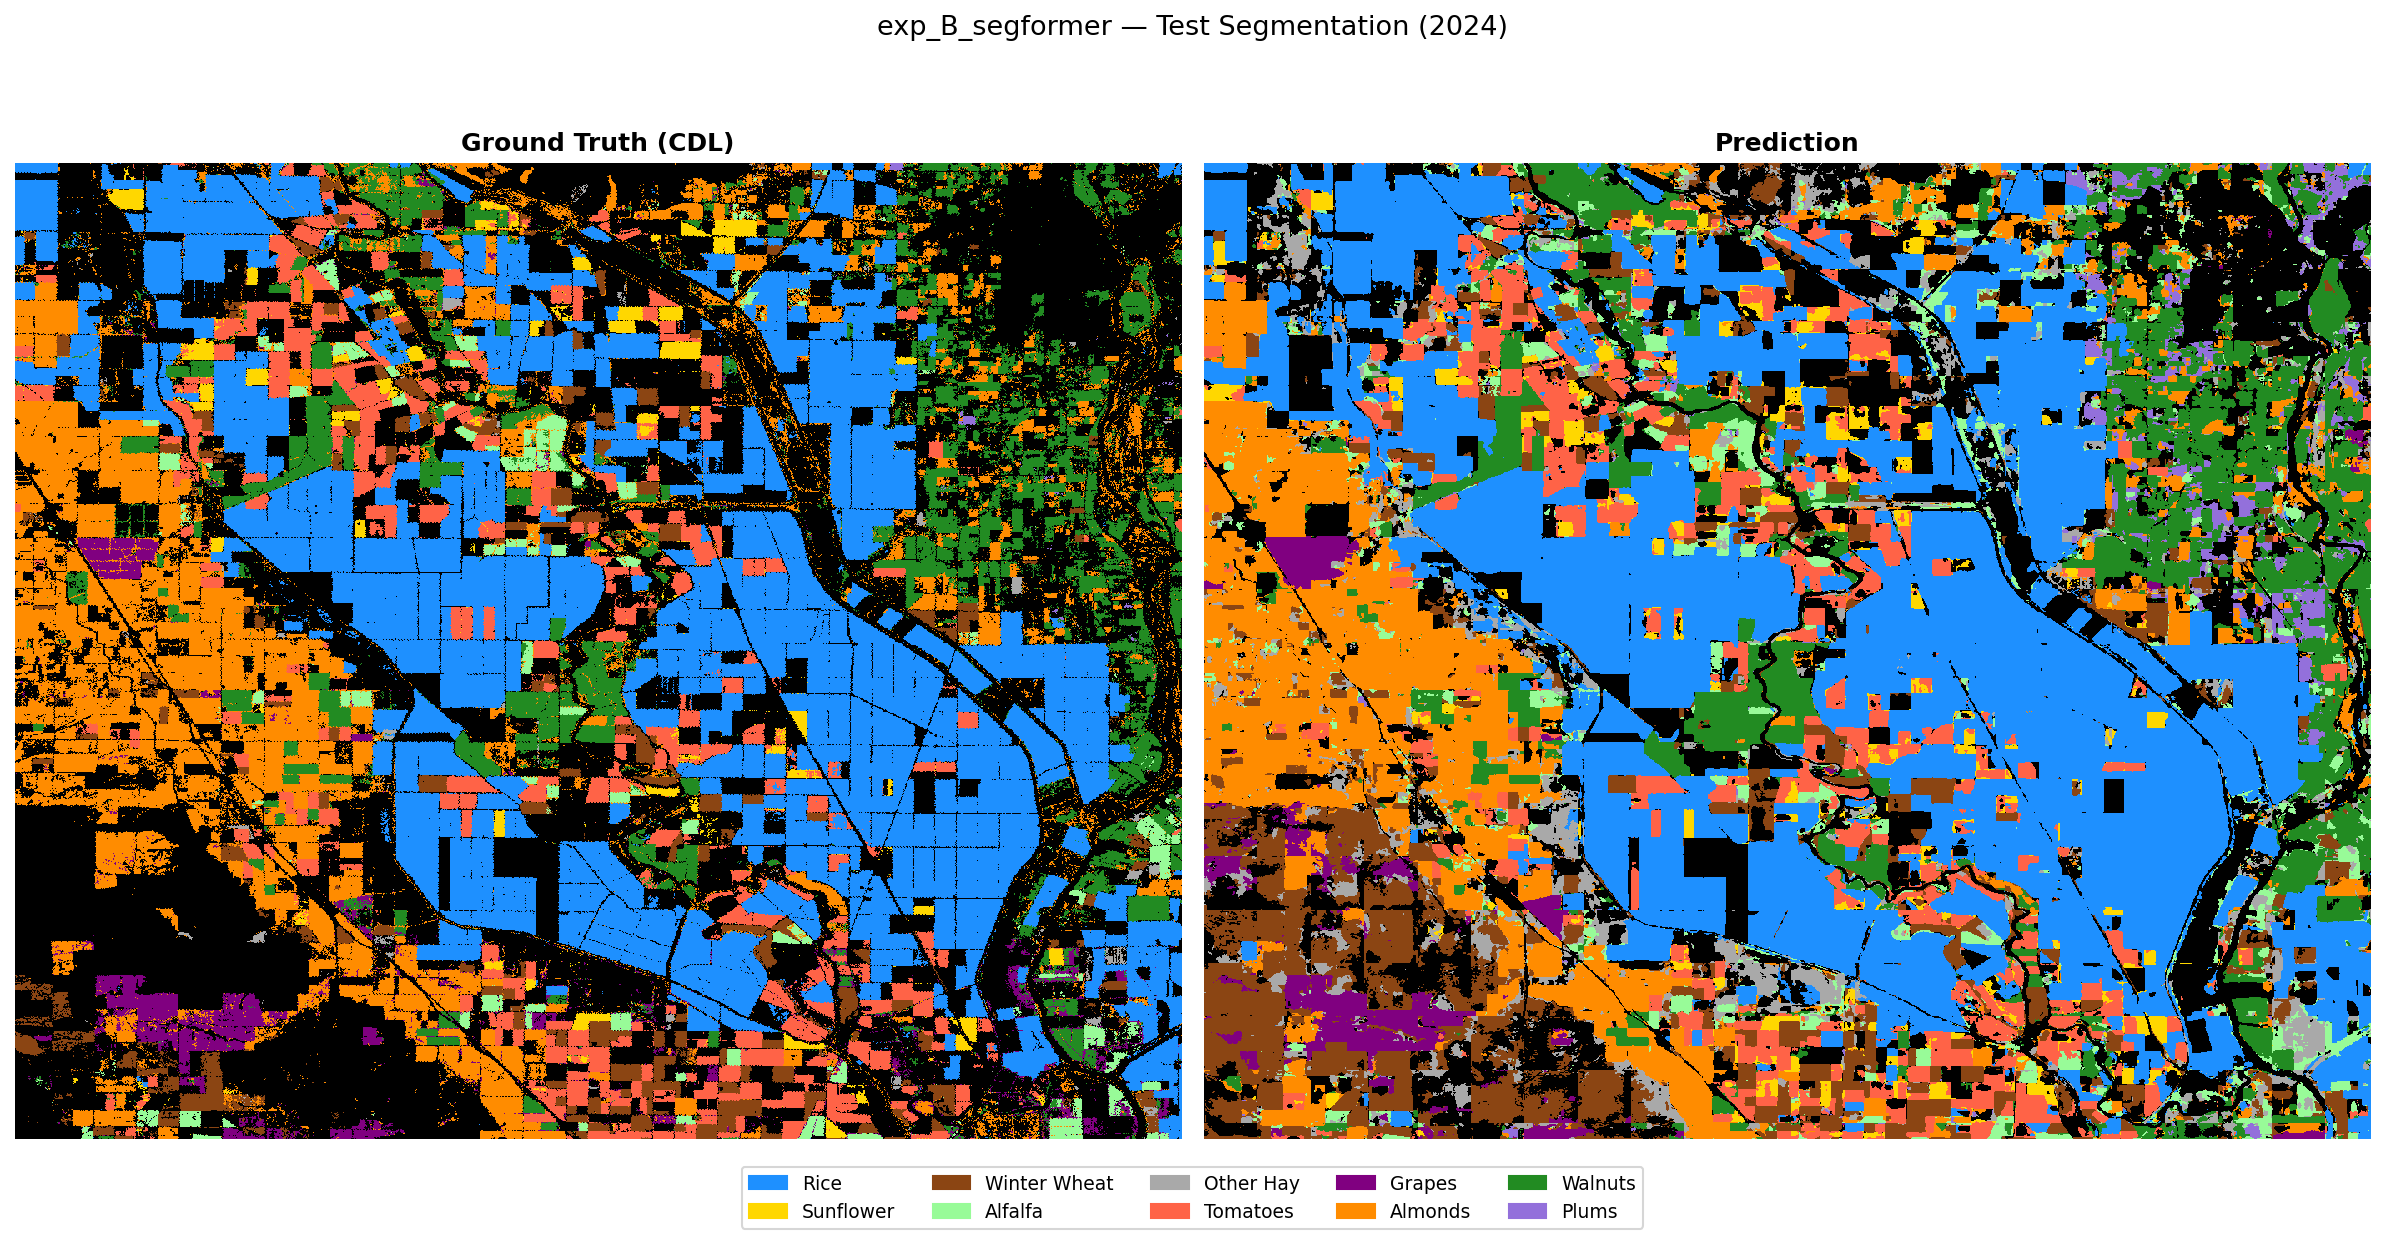
\includegraphics[width=\textwidth]{figures/sf_expb_map.png}
        \caption{Exp B --- \textit{Multi-Temporal} Naif (36 ch)}
    \end{subfigure}
    \vspace{1em}
    \begin{subfigure}{0.85\textwidth}
        \centering
        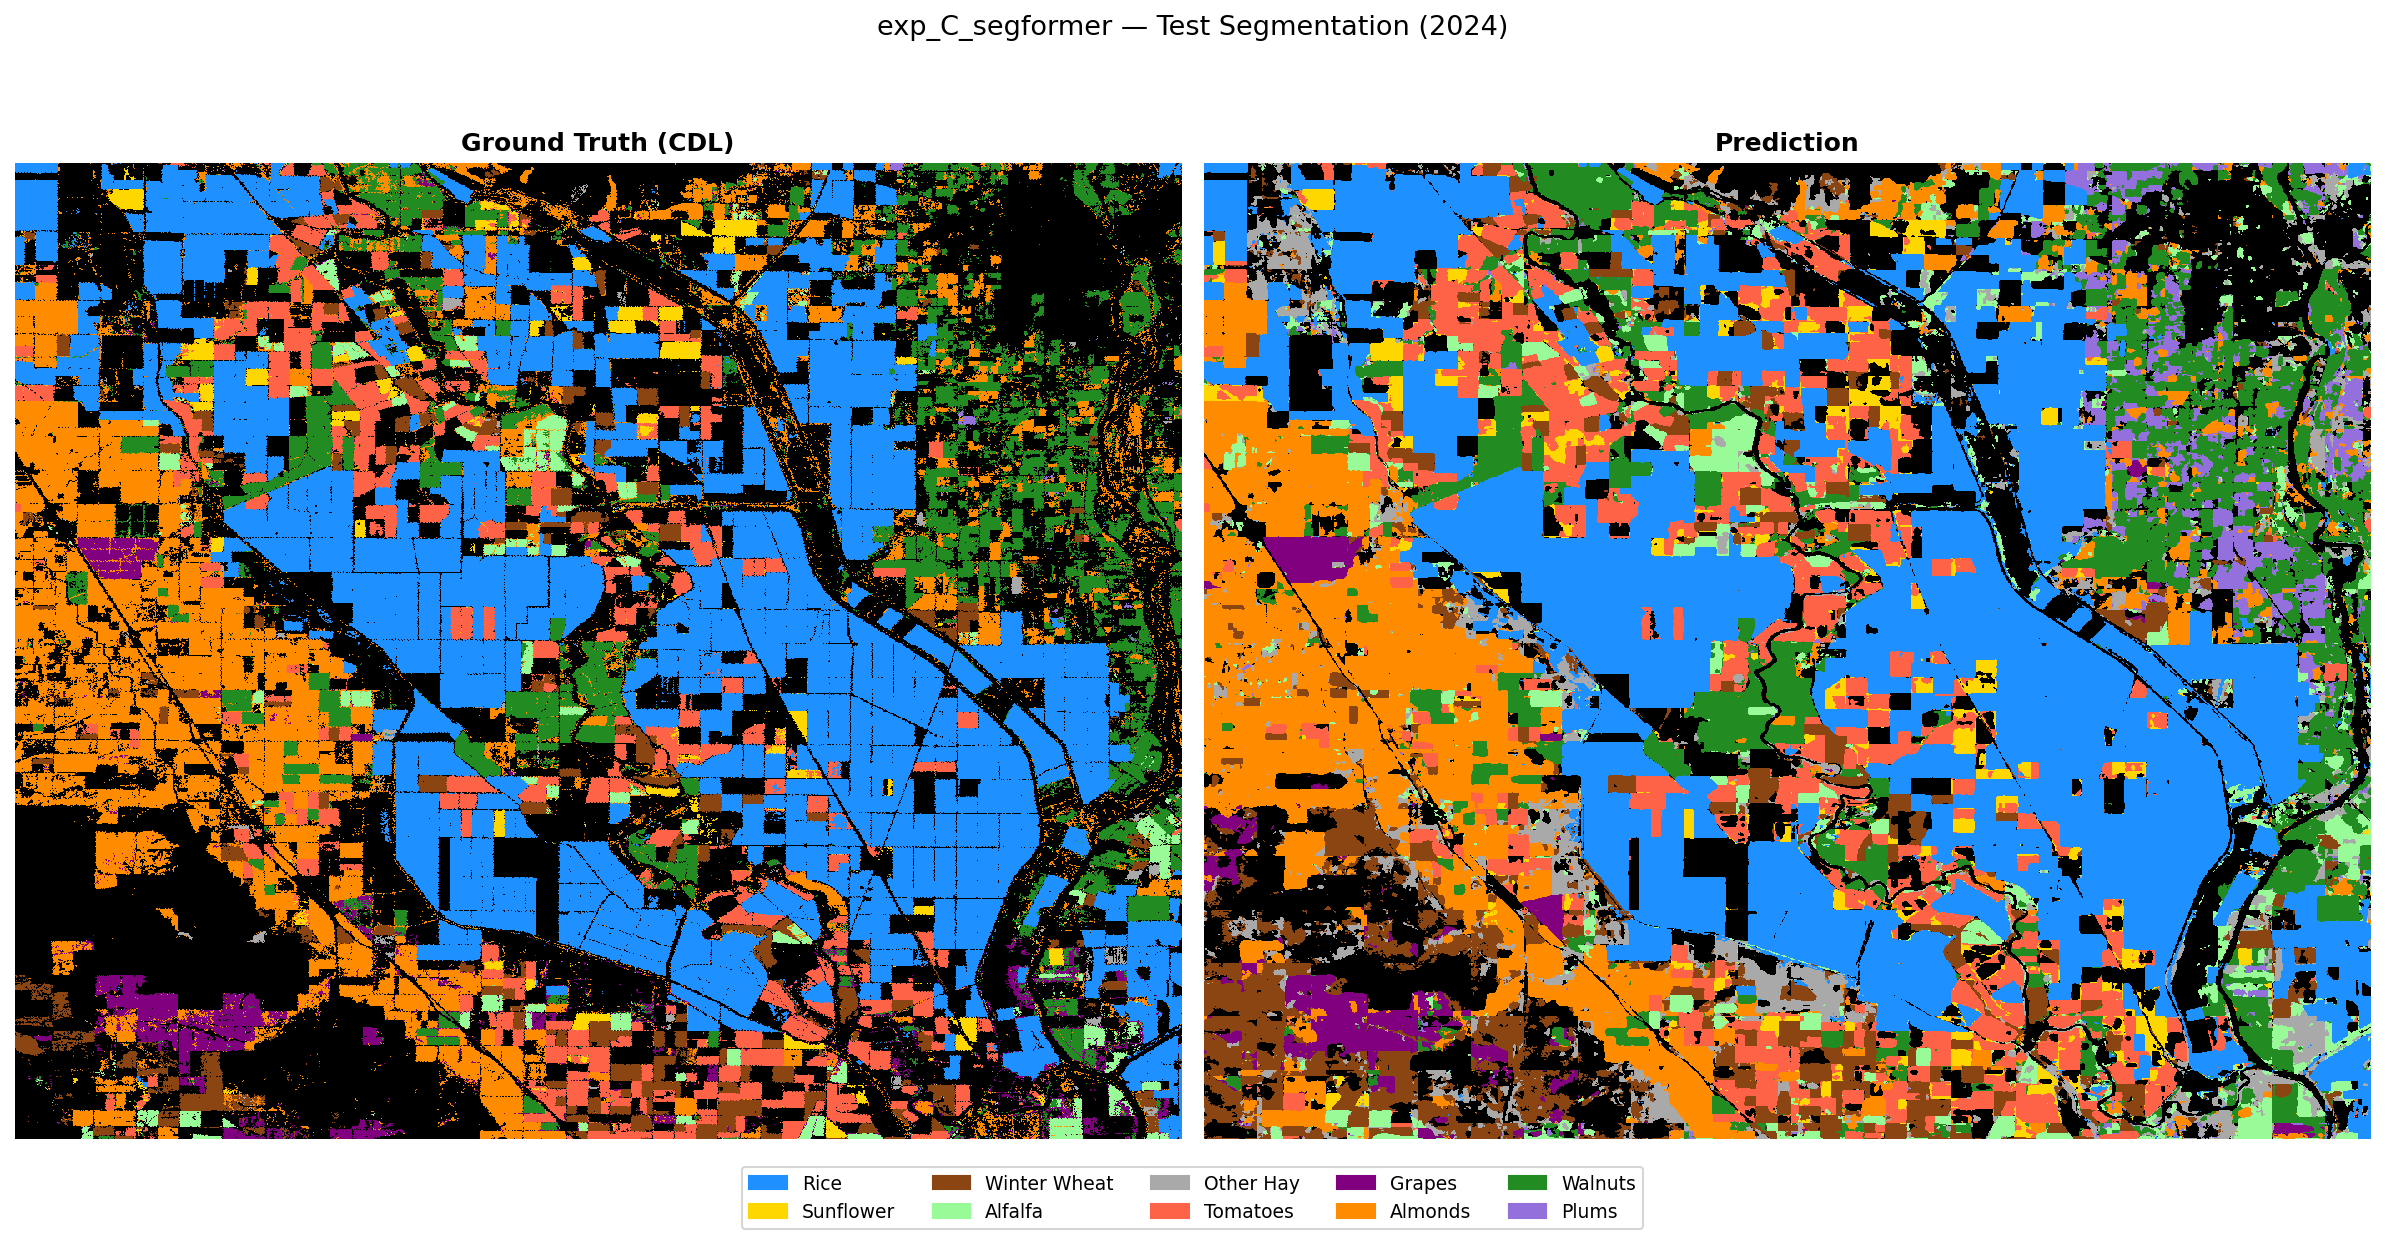
\includegraphics[width=\textwidth]{figures/sf_expc_map.png}
        \caption{Exp C\_v3 --- Band $k$=5 (39 ch, SegFormer terbaik Phase A)}
    \end{subfigure}
    \caption{Peta segmentasi penuh set uji 2024 menggunakan SegFormer.}
    \label{fig:seg_results_sf}
\end{figure}
